% ===========================================================================
%  Verteidigungsvortrag zur Bachelorarbeit
%  "Datenaugmentierung fuer die CNN-basierte Detektion von
%   Rohrprofil-Stirnflaechen an gestapelten Bauzaunfeldern"
%
%  ENTWURFSPRINZIP: eine Aussage pro Folie, gross gesetzt.  Die Folien tragen
%  nur den Anker, an dem der Satz haengt; die Prosa steht im Sprechtext
%  (\note) und die Belege auf den Zusatzfolien im Anhang.  Das Hoehenbudget
%  je Folie und die erlaubten Bauformen stehen in vortrag_stil.tex.
%
%  Alle Messzahlen kommen aus kapitel/zahlen.tex -- derselben Datei, die
%  main.tex einliest und die src/report_neu.py schreibt.  Die Folien koennen
%  deshalb nicht von der Arbeit abweichen.
%
%  Uebersetzen:  make vortrag            (nur Folien)
%                make vortrag-pruefen    (nennt Folien, die zu voll sind)
%                make vortrag-notizen    (Folie links, Sprechnotiz rechts)
%
%  Ablaufplan und vorbereitete Antworten: VORTRAG.md
% ===========================================================================
\documentclass[14pt,aspectratio=169]{beamer}

% ===========================================================================
%  Stil des Verteidigungsvortrags -- von vortrag.tex geladen.
%
%  Leitgedanke: EINE Aussage pro Folie, gross gesetzt.  Die Grundschrift ist
%  deshalb die 14pt-Klasse und nicht 10 oder 11pt; Aufzaehlungen laufen in
%  \large.  Was hier nicht als Makro vorgesehen ist, gehoert nicht auf eine
%  Folie, sondern in den Sprechtext (\note) oder auf eine Zusatzfolie.
%
%  Die mitgelieferten beamer-Themen bringen Navigationsleisten und
%  Schattenkaesten mit, die auf einem Projektor nur Platz kosten -- deshalb
%  das Standardthema als Grundlage und alles Sichtbare hier definiert.
% ===========================================================================
\usetheme{default}
\usecolortheme{default}
\setbeamertemplate{navigation symbols}{}

\usepackage{iftex}
\ifPDFTeX
  \usepackage[utf8]{inputenc}
  \usepackage[T1]{fontenc}
  \usepackage{lmodern}
\else
  \usepackage{fontspec}
\fi
\usepackage[ngerman]{babel}
\usepackage[german=quotes]{csquotes}
\usepackage{amsmath,amssymb}
\usepackage{booktabs}
\usepackage{array}
\usepackage{graphicx}
\usepackage{tikz}
\usetikzlibrary{arrows.meta,positioning,calc,fit}
\usepackage{appendixnumberbeamer}

% --------------------------------------------------------------------------
%  Farben.  akzent traegt Titel und Hervorhebung, gut/warn die Richtung eines
%  Effekts, die Belegart-Marker die Beweislage.
% --------------------------------------------------------------------------
\definecolor{akzent}{RGB}{20,64,116}
\definecolor{akzenthell}{RGB}{72,124,180}
\definecolor{gut}{RGB}{22,110,60}
\definecolor{warn}{RGB}{176,58,20}
\definecolor{grau}{RGB}{115,115,115}
\definecolor{hgrau}{RGB}{243,244,246}

\setbeamercolor{structure}{fg=akzent}
\setbeamercolor{frametitle}{fg=akzent,bg=}
\setbeamercolor{framesubtitle}{fg=grau,bg=}
\setbeamercolor{footline}{fg=grau}
\setbeamercolor{alerted text}{fg=warn}

\setbeamerfont{frametitle}{size=\Large,series=\bfseries}
\setbeamerfont{framesubtitle}{size=\normalsize,series=\mdseries}
\setbeamerfont{footline}{size=\tiny}
\setbeamerfont{itemize/enumerate body}{size=\large}
\setbeamerfont{itemize/enumerate subbody}{size=\normalsize}
\setbeamerfont{description item}{series=\bfseries}

% Flache Striche statt Kugeln: laeuft bei grosser Schrift ruhiger.
\newcommand{\markerI}{\color{akzenthell}\rule[0.30ex]{0.55em}{1.1pt}}
\newcommand{\markerII}{\color{grau}\rule[0.30ex]{0.38em}{0.8pt}}
\setbeamertemplate{itemize item}{\markerI}
\setbeamertemplate{itemize subitem}{\markerII}
\setbeamertemplate{enumerate item}{\color{akzent}\bfseries\insertenumlabel.}

\setbeamersize{text margin left=1.1em,text margin right=1.1em}

% Die Aufzaehlung des Hauptteils.  Bei 14pt-Grundschrift kleben Punkte mit
% dem beamer-Standardabstand aneinander; enumitem waere der uebliche Weg,
% bricht aber beamers \insertenumlabel (\labelenumi -> {\labelenumi},
% Endlosrekursion).  Deshalb eine eigene Liste: der Abstand ist damit exakt
% bekannt, und genau darauf stuetzt sich das Hoehenbudget weiter unten.
%   \begin{punkte}          Hauptteil, luftig
%   \begin{punkte}[0.25em]  Zusatzfolien, dicht
\newenvironment{punkte}[1][0.55em]{%
  \begin{list}{\markerI}{%
    \setlength{\leftmargin}{1.6em}%
    \setlength{\labelwidth}{0.8em}%
    \setlength{\labelsep}{0.7em}%
    \setlength{\itemsep}{#1}%
    \setlength{\parsep}{0pt}%
    \setlength{\topsep}{0.4em}%
    \setlength{\partopsep}{0pt}%
  }}{\end{list}}

% --------------------------------------------------------------------------
%  Folientitel mit Trennlinie, Fusszeile mit Abschnitt und Foliennummer.
% --------------------------------------------------------------------------
\makeatletter
\setbeamertemplate{frametitle}{%
  \nointerlineskip\vskip0.85em%
  \begin{beamercolorbox}[wd=\paperwidth,leftskip=\beamer@leftmargin,
                         rightskip=\beamer@rightmargin]{frametitle}%
    \usebeamerfont{frametitle}\insertframetitle%
    \ifx\insertframesubtitle\@empty\else%
      \\[0.2em]{\usebeamerfont{framesubtitle}%
        \usebeamercolor[fg]{framesubtitle}\insertframesubtitle}%
    \fi%
    \\[0.3em]{\color{akzent!22}\rule{\dimexpr\paperwidth-\beamer@leftmargin-\beamer@rightmargin\relax}{1pt}}%
  \end{beamercolorbox}%
  \vskip0.6em%
}
\setbeamertemplate{footline}{%
  \begin{beamercolorbox}[wd=\paperwidth,ht=2.4ex,dp=1.6ex,
                         leftskip=\beamer@leftmargin,
                         rightskip=\beamer@rightmargin]{footline}%
    \usebeamerfont{footline}%
    \insertshorttitle\hfill\insertsectionhead\hfill%
    \insertframenumber\,/\,\inserttotalframenumber%
  \end{beamercolorbox}%
}
\makeatother

% --------------------------------------------------------------------------
%  Makros -- dieselben Namen wie in praeambel.tex, damit Textbausteine und
%  Zahlen aus kapitel/ unveraendert uebernommen werden koennen.
% --------------------------------------------------------------------------
\newcommand{\code}[1]{\texttt{#1}}
\newcommand{\px}{\,px}
\newcommand{\PP}{\,\textnormal{\%-Punkte}}  % \textnormal, damit der Bindestrich
                                            % im Mathemodus kein Minus wird
\newcommand{\mAPfifty}{mAP@0{,}5}
\newcommand{\mAPseven}{mAP@0{,}75}
\newcommand{\mAPall}{mAP@0{,}5{:}0{,}95}
\newcommand{\Oe}{\ensuremath{\varnothing}}
\newcolumntype{L}[1]{>{\raggedright\arraybackslash}p{#1}}
\newcolumntype{R}[1]{>{\raggedleft\arraybackslash}p{#1}}

% Belegart: M gemessen, P physikalisch, L Literatur, A Annahme.
\newcommand{\bM}{\textcolor{gut}{\textbf{M}}}
\newcommand{\bP}{\textcolor{akzent}{\textbf{P}}}
\newcommand{\bL}{\textcolor{akzenthell}{\textbf{L}}}
\newcommand{\bA}{\textcolor{warn}{\textbf{A}}}

% --------------------------------------------------------------------------
%  Das Hoehenbudget einer Folie -- an dieser Klasse gemessen, nicht geschaetzt.
%
%  \textheight ist 241 pt, \textwidth 425 pt (14,97 cm).  Davon gehen ab:
%    Folientitel ohne Untertitel   ~50 pt      Fusszeile   ~14 pt
%    Folientitel mit  Untertitel   ~71 pt
%  Es bleiben also 177 pt (ohne Untertitel) bzw. 156 pt (mit Untertitel).
%
%  Was das kostet:
%    ein Aufzaehlungspunkt (\large, einzeilig)   22 pt  + 9 pt Abstand
%    eine Umbruchzeile darin                     22 pt
%    \fuss{}                                    ~34 pt
%    \grosszahl{}{}{}                           ~124 pt
%    \zweizahl{}{}{}{}                           ~89 pt
%    \botschaft{} je Zeile                       ~39 pt
%
%  Daraus die Obergrenzen, die beim Schreiben gelten:
%    mit Untertitel     4 Punkte   ODER 3 Punkte + \fuss
%    ohne Untertitel    5 Punkte   ODER 4 Punkte + \fuss
%    Grosszahl + \fuss  nur ohne Untertitel
%
%  Wer mehr braucht, hat zwei Folien -- nicht eine kleinere Schrift.
%  'make vortrag-pruefen' nennt jede Folie, die die Grenze reisst.
% --------------------------------------------------------------------------

% --------------------------------------------------------------------------
%  Folientypen.  Jeder steht fuer genau eine Art von Aussage; zusammen sind
%  sie die einzigen erlaubten Bauformen einer Folie im Hauptteil.
% --------------------------------------------------------------------------

% (1) Botschaft: ein Satz, der die Folie ganz fuellt.  Fuer die Kernsaetze.
\newcommand{\botschaft}[1]{%
  \vfill
  {\LARGE\baselineskip=1.35\baselineskip\color{akzent}#1\par}
  \vfill}

% (2) Grosszahl: die Zahl ist der Inhalt, nicht ihre Tabellenzeile.
%     #1 Wert, #2 Beschriftung, #3 Zusatz (darf leer sein)
\newcommand{\grosszahl}[3]{%
  \begin{center}
    {\fontsize{62}{66}\selectfont\bfseries\color{akzent}#1}\\[0.35em]
    {\Large #2}%
    \ifx\relax#3\relax\else\\[0.2em]{\normalsize\color{grau}#3}\fi
  \end{center}}

% (3) Zwei Zahlen nebeneinander -- fuer val gegen test.
\newcommand{\zweizahl}[4]{%
  \begin{center}
  \begin{minipage}{0.46\textwidth}\centering
    {\fontsize{56}{62}\selectfont\bfseries\color{akzent}#1}\\[0.35em]{\large #2}
  \end{minipage}\hfill
  \begin{minipage}{0.46\textwidth}\centering
    {\fontsize{56}{62}\selectfont\bfseries\color{akzent}#3}\\[0.35em]{\large #4}
  \end{minipage}
  \end{center}}

% (3b) Drei Zahlen -- fuer das verfuegbare Quellmaterial 9 / 7 / 2.
\newcommand{\dreizahl}[6]{%
  \begin{center}
  \begin{minipage}{0.30\textwidth}\centering
    {\fontsize{54}{60}\selectfont\bfseries\color{akzent}#1}\\[0.3em]{\large #2}
  \end{minipage}\hfill
  \begin{minipage}{0.30\textwidth}\centering
    {\fontsize{54}{60}\selectfont\bfseries\color{akzent}#3}\\[0.3em]{\large #4}
  \end{minipage}\hfill
  \begin{minipage}{0.30\textwidth}\centering
    {\fontsize{54}{60}\selectfont\bfseries\color{akzent}#5}\\[0.3em]{\large #6}
  \end{minipage}
  \end{center}}

% (3c) Von-nach-Zahl: der Effekt ist der Sprung, nicht der Endwert.
\newcommand{\sprungzahl}[5]{%
  \begin{center}
    {\Large\color{grau}#1}\quad
    {\fontsize{42}{46}\selectfont\bfseries\color{grau}#2}\;
    {\fontsize{42}{46}\selectfont\color{akzenthell}$\rightarrow$}\;
    {\fontsize{42}{46}\selectfont\bfseries\color{akzent}#3}\\[0.4em]
    {\Large #4}%
    \ifx\relax#5\relax\else\\[0.2em]{\normalsize\color{grau}#5}\fi
  \end{center}}

% (3d) Schlagwortreihe: sechs Begriffe als Inhalt, ohne Erklaerung.
%      Die Erklaerung steht im Sprechtext und auf der Zusatzfolie.
\newcommand{\schlagworte}[1]{%
  \begin{center}\large
    \begingroup\setlength{\tabcolsep}{0.55em}#1\endgroup
  \end{center}}

% (4) Fussnotiz einer Folie: die eine Einschraenkung, die dazugehoert.
%     Bewusst klein und grau -- sie ist Beiwerk, nicht Inhalt.
% Regel: hoechstens zwei Zeilen.  Wer drei braucht, gehoert in den
% Sprechtext -- \fuss traegt eine Einschraenkung, nie ein Argument.
\newcommand{\fuss}[1]{%
  \par\vspace{0.5em}
  {\color{akzent!18}\rule{0.30\linewidth}{0.7pt}}\par\vspace{0.25em}
  {\footnotesize\color{grau}#1\par}}

% (4b) Abbildung mit Hoehendeckel.  \bild deckelt auf eine Hoehe, die mit
%      Titel UND \fuss noch passt; \bildgross auf eine, die ohne \fuss passt.
%      keepaspectratio, damit breite Plots an der Breite und hohe Fotos an
%      der Hoehe begrenzt werden.
\newcommand{\bild}[1]{%
  \begingroup\centering
    \includegraphics[width=\textwidth,height=0.50\textheight,
                     keepaspectratio]{#1}\par
  \endgroup}
\newcommand{\bildgross}[1]{%
  \begingroup\centering
    \includegraphics[width=\textwidth,height=0.54\textheight,
                     keepaspectratio]{#1}\par
  \endgroup}

% (5) Abschnittstrenner.
\newcommand{\trenner}[2]{%
  \begin{frame}[plain,noframenumbering]
    \vfill
    \begin{center}
      {\color{grau}\large #1}\\[0.5em]
      {\color{akzent}\Huge\bfseries #2}
    \end{center}
    \vfill
  \end{frame}}

% (6) Hervorgehobener Kasten fuer eine einzelne kurze Aussage.
\newcommand{\kasten}[1]{%
  \begingroup\setlength{\fboxsep}{0.7em}%
  \noindent\colorbox{hgrau}{\begin{minipage}{\dimexpr\linewidth-1.4em\relax}%
    \centering#1%
  \end{minipage}}\endgroup}

% (7) Budgetmarker.  Alle drei Entwuerfe nannten dasselbe Risiko: Auf den
%     Ablationsfolien liegen 0,961 und 0,969 nur wenige Folien auseinander,
%     stammen aber aus verschiedenen Budgets.  Der Marker steht deshalb auf
%     JEDER Ablationsfolie an derselben Stelle.
\newcommand{\budgetmarker}{%
  \par\nointerlineskip
  \hfill\raisebox{0pt}[0pt][0pt]{%
    \colorbox{hgrau}{\footnotesize\color{grau}%
      \,3000 Bilder $\cdot$ 30 Epochen $\cdot$ nicht mit dem Referenzmodell
      vergleichbar\,}}\par\nointerlineskip}

% Zusatzfolien im Anhang duerfen dicht sein -- sie werden nur in der
% Diskussion gezeigt und dann gelesen, nicht vorgetragen.
% Referenzmaterial, aus der Naehe gelesen -- nicht projizierte Prosa.
\newcommand{\zusatzdicht}{\fontsize{7.5}{9}\selectfont}


%% Notizfassung -- von aussen ueber \def\NOTIZEN{} eingeschaltet.
\ifdefined\NOTIZEN
  \usepackage{pgfpages}
  \setbeameroption{show notes on second screen=right}
\fi

%% Alle Messzahlen, geteilt mit main.tex.
% Automatisch erzeugt von src/report_neu.py -- nicht von Hand
% bearbeiten. Jede im Fliesstext genannte Messzahl steht hier.

\newcommand{\zAOneEpoche}{28}
\newcommand{\zAOneLabels}{68\,281}
\newcommand{\zAOneTestCnt}{87}
\newcommand{\zAOneTestFf}{0{,}932}
\newcommand{\zAOneTestMap}{0{,}961}
\newcommand{\zAOneTestMapA}{0{,}481}
\newcommand{\zAOneTestPrec}{0{,}943}
\newcommand{\zAOneTestRec}{0{,}921}
\newcommand{\zAOneValCnt}{99}
\newcommand{\zAOneValFf}{0{,}944}
\newcommand{\zAOneValMap}{0{,}974}
\newcommand{\zAOneValMapA}{0{,}647}
\newcommand{\zAOneValPrec}{0{,}939}
\newcommand{\zAOneValRec}{0{,}949}
\newcommand{\zATwoEpoche}{29}
\newcommand{\zATwoLabels}{55\,833}
\newcommand{\zATwoTestCnt}{95}
\newcommand{\zATwoTestFf}{0{,}924}
\newcommand{\zATwoTestMap}{0{,}964}
\newcommand{\zATwoTestMapA}{0{,}457}
\newcommand{\zATwoTestPrec}{0{,}895}
\newcommand{\zATwoTestRec}{0{,}955}
\newcommand{\zATwoValCnt}{96}
\newcommand{\zATwoValFf}{0{,}938}
\newcommand{\zATwoValMap}{0{,}957}
\newcommand{\zATwoValMapA}{0{,}617}
\newcommand{\zATwoValPrec}{0{,}948}
\newcommand{\zATwoValRec}{0{,}929}
\newcommand{\zAZeroEpoche}{21}
\newcommand{\zAZeroLabels}{82\,950}
\newcommand{\zAZeroTestCnt}{81}
\newcommand{\zAZeroTestFf}{0{,}929}
\newcommand{\zAZeroTestMap}{0{,}958}
\newcommand{\zAZeroTestMapA}{0{,}506}
\newcommand{\zAZeroTestPrec}{0{,}975}
\newcommand{\zAZeroTestRec}{0{,}888}
\newcommand{\zAZeroValCnt}{89}
\newcommand{\zAZeroValFf}{0{,}909}
\newcommand{\zAZeroValMap}{0{,}953}
\newcommand{\zAZeroValMapA}{0{,}638}
\newcommand{\zAZeroValPrec}{0{,}955}
\newcommand{\zAZeroValRec}{0{,}867}
\newcommand{\zBOneEpoche}{20}
\newcommand{\zBOneLabels}{68\,281}
\newcommand{\zBOneTestCnt}{81}
\newcommand{\zBOneTestFf}{0{,}941}
\newcommand{\zBOneTestFn}{9}
\newcommand{\zBOneTestMap}{0{,}963}
\newcommand{\zBOneTestMapA}{0{,}481}
\newcommand{\zBOneTestPrec}{0{,}988}
\newcommand{\zBOneTestRec}{0{,}899}
\newcommand{\zBOneTestRecGross}{0{,}966}
\newcommand{\zBOneTestRecKlein}{0{,}767}
\newcommand{\zBOneValCnt}{97}
\newcommand{\zBOneValFf}{0{,}913}
\newcommand{\zBOneValFn}{9}
\newcommand{\zBOneValMap}{0{,}944}
\newcommand{\zBOneValMapA}{0{,}585}
\newcommand{\zBOneValPrec}{0{,}918}
\newcommand{\zBOneValRec}{0{,}908}
\newcommand{\zBOneValRecGross}{0{,}938}
\newcommand{\zBOneValRecKlein}{0{,}848}
\newcommand{\zBTwoEpoche}{15}
\newcommand{\zBTwoLabels}{68\,281}
\newcommand{\zBTwoTestCnt}{76}
\newcommand{\zBTwoTestFf}{0{,}885}
\newcommand{\zBTwoTestFn}{16}
\newcommand{\zBTwoTestMap}{0{,}914}
\newcommand{\zBTwoTestMapA}{0{,}470}
\newcommand{\zBTwoTestPrec}{0{,}961}
\newcommand{\zBTwoTestRec}{0{,}820}
\newcommand{\zBTwoTestRecGross}{0{,}949}
\newcommand{\zBTwoTestRecKlein}{0{,}567}
\newcommand{\zBTwoValCnt}{95}
\newcommand{\zBTwoValFf}{0{,}922}
\newcommand{\zBTwoValFn}{9}
\newcommand{\zBTwoValMap}{0{,}964}
\newcommand{\zBTwoValMapA}{0{,}654}
\newcommand{\zBTwoValPrec}{0{,}937}
\newcommand{\zBTwoValRec}{0{,}908}
\newcommand{\zBTwoValRecGross}{0{,}923}
\newcommand{\zBTwoValRecKlein}{0{,}879}
\newcommand{\zBZeroEpoche}{28}
\newcommand{\zBZeroLabels}{68\,281}
\newcommand{\zBZeroTestCnt}{87}
\newcommand{\zBZeroTestFf}{0{,}932}
\newcommand{\zBZeroTestFn}{7}
\newcommand{\zBZeroTestMap}{0{,}961}
\newcommand{\zBZeroTestMapA}{0{,}481}
\newcommand{\zBZeroTestPrec}{0{,}943}
\newcommand{\zBZeroTestRec}{0{,}921}
\newcommand{\zBZeroTestRecGross}{0{,}983}
\newcommand{\zBZeroTestRecKlein}{0{,}800}
\newcommand{\zBZeroValCnt}{99}
\newcommand{\zBZeroValFf}{0{,}944}
\newcommand{\zBZeroValFn}{5}
\newcommand{\zBZeroValMap}{0{,}974}
\newcommand{\zBZeroValMapA}{0{,}647}
\newcommand{\zBZeroValPrec}{0{,}939}
\newcommand{\zBZeroValRec}{0{,}949}
\newcommand{\zBZeroValRecGross}{0{,}969}
\newcommand{\zBZeroValRecKlein}{0{,}909}
\newcommand{\zCOneLabels}{67\,727}
\newcommand{\zCOneSval}{0{,}978}
\newcommand{\zCOneSvalFf}{0{,}947}
\newcommand{\zCOneTestCnt}{76}
\newcommand{\zCOneTestFf}{0{,}800}
\newcommand{\zCOneTestMap}{0{,}835}
\newcommand{\zCOneTestMapA}{0{,}328}
\newcommand{\zCOneTestPrec}{0{,}868}
\newcommand{\zCOneTestRec}{0{,}742}
\newcommand{\zCOneValCnt}{91}
\newcommand{\zCOneValFf}{0{,}825}
\newcommand{\zCOneValMap}{0{,}867}
\newcommand{\zCOneValMapA}{0{,}557}
\newcommand{\zCOneValPrec}{0{,}857}
\newcommand{\zCOneValRec}{0{,}796}
\newcommand{\zCZeroLabels}{68\,280}
\newcommand{\zCZeroSval}{0{,}982}
\newcommand{\zCZeroSvalFf}{0{,}966}
\newcommand{\zCZeroTestCnt}{88}
\newcommand{\zCZeroTestFf}{0{,}904}
\newcommand{\zCZeroTestMap}{0{,}948}
\newcommand{\zCZeroTestMapA}{0{,}463}
\newcommand{\zCZeroTestPrec}{0{,}909}
\newcommand{\zCZeroTestRec}{0{,}899}
\newcommand{\zCZeroValCnt}{94}
\newcommand{\zCZeroValFf}{0{,}917}
\newcommand{\zCZeroValMap}{0{,}947}
\newcommand{\zCZeroValMapA}{0{,}620}
\newcommand{\zCZeroValPrec}{0{,}936}
\newcommand{\zCZeroValRec}{0{,}898}
\newcommand{\zablALabelDrop}{32{,}7}
\newcommand{\zablATestGain}{-0{,}5}
\newcommand{\zablAValGain}{0{,}4}
\newcommand{\zablBTestGap}{4{,}7}
\newcommand{\zablBTestGapEins}{-0{,}2}
\newcommand{\zablBTestGapFf}{4{,}7}
\newcommand{\zablBTestGapRec}{10{,}1}
\newcommand{\zablBValGap}{1{,}0}
\newcommand{\zablBValGapEins}{3{,}0}
\newcommand{\zablCLabelDiff}{553}
\newcommand{\zablCLabelDiffProz}{0{,}8}
\newcommand{\zablCSvalGap}{-0{,}4}
\newcommand{\zablCTestGap}{-11{,}3}
\newcommand{\zablCTestGapFf}{-10{,}4}
\newcommand{\zablCTestGapRec}{-15{,}7}
\newcommand{\zablCValGap}{-8{,}0}
\newcommand{\zablCValGapFf}{-9{,}1}
\newcommand{\zablCValGapRec}{-10{,}2}
\newcommand{\zbestImgsz}{1920}
\newcommand{\zbootTestHi}{0{,}982}
\newcommand{\zbootTestLo}{0{,}921}
\newcommand{\zbootTestMean}{0{,}952}
\newcommand{\zbootTestN}{22}
\newcommand{\zbootTestStd}{0{,}016}
\newcommand{\zbootValHi}{0{,}969}
\newcommand{\zbootValLo}{0{,}891}
\newcommand{\zbootValMean}{0{,}934}
\newcommand{\zbootValN}{21}
\newcommand{\zbootValStd}{0{,}020}
\newcommand{\zboxSvalCtr}{0{,}021}
\newcommand{\zboxSvalGross}{0{,}999}
\newcommand{\zboxSvalKlein}{1{,}015}
\newcommand{\zboxSvalOff}{-0{,}08}
\newcommand{\zboxSvalPaare}{7224}
\newcommand{\zboxSvalRatio}{1{,}003}
\newcommand{\zboxTestCtr}{0{,}051}
\newcommand{\zboxTestGross}{0{,}904}
\newcommand{\zboxTestKlein}{0{,}896}
\newcommand{\zboxTestOff}{2{,}00}
\newcommand{\zboxTestPaare}{88}
\newcommand{\zboxTestRatio}{0{,}897}
\newcommand{\zboxValCtr}{0{,}056}
\newcommand{\zboxValGross}{0{,}932}
\newcommand{\zboxValOff}{1{,}58}
\newcommand{\zboxValPaare}{97}
\newcommand{\zboxValRatio}{0{,}944}
\newcommand{\zepsDiff}{0{,}015}
\newcommand{\zepsS}{0{,}016}
\newcommand{\zepsT}{0{,}031}
\newcommand{\zfnKleinTest}{7}
\newcommand{\zfnKleinVal}{2}
\newcommand{\zfnMaxTest}{21{,}7}
\newcommand{\zfnMaxVal}{33{,}9}
\newcommand{\zfnTest}{8}
\newcommand{\zfnVal}{12}
\newcommand{\zfpDoppelTest}{3}
\newcommand{\zfpDoppelVal}{3}
\newcommand{\zfpOhneTest}{0}
\newcommand{\zfpOhneVal}{1}
\newcommand{\zfpTest}{3}
\newcommand{\zfpVal}{5}
\newcommand{\zgapCOneTest}{14{,}2}
\newcommand{\zgapCOneVal}{11{,}1}
\newcommand{\zgapCZeroTest}{3{,}4}
\newcommand{\zgapCZeroVal}{3{,}5}
\newcommand{\zgrenzeTest}{14{,}9}
\newcommand{\zgrenzeVal}{25{,}4}
\newcommand{\znGrossTest}{59}
\newcommand{\znGrossVal}{65}
\newcommand{\znKleinTest}{30}
\newcommand{\znKleinVal}{33}
\newcommand{\znPredTest}{84}
\newcommand{\znPredVal}{91}
\newcommand{\znmsAbstandMin}{0{,}043}
\newcommand{\znmsAnteil}{2{,}3}
\newcommand{\znmsIouMax}{0{,}981}
\newcommand{\znmsIouMin}{0{,}892}
\newcommand{\znmsKopien}{4}
\newcommand{\znmsTestAbstandMin}{0{,}043}
\newcommand{\znmsTestBoxenMit}{81}
\newcommand{\znmsTestBoxenOhne}{84}
\newcommand{\znmsTestEntfernt}{3}
\newcommand{\znmsTestFfMit}{0{,}953}
\newcommand{\znmsTestFfOhne}{0{,}936}
\newcommand{\znmsTestFn}{8}
\newcommand{\znmsTestFpMit}{0}
\newcommand{\znmsTestFpOhne}{3}
\newcommand{\znmsTestGain}{1{,}7}
\newcommand{\znmsTestIouMax}{0{,}974}
\newcommand{\znmsTestIouMin}{0{,}892}
\newcommand{\znmsTestTp}{81}
\newcommand{\znmsValAbstandMin}{0{,}230}
\newcommand{\znmsValBoxenMit}{90}
\newcommand{\znmsValBoxenOhne}{91}
\newcommand{\znmsValEntfernt}{1}
\newcommand{\znmsValFfMit}{0{,}915}
\newcommand{\znmsValFfOhne}{0{,}910}
\newcommand{\znmsValFn}{12}
\newcommand{\znmsValFpMit}{4}
\newcommand{\znmsValFpOhne}{5}
\newcommand{\znmsValGain}{0{,}5}
\newcommand{\znmsValIouMax}{0{,}981}
\newcommand{\znmsValIouMin}{0{,}981}
\newcommand{\znmsValTp}{86}
\newcommand{\znmsVorhersagen}{175}
\newcommand{\zrefBestEpoche}{23}
\newcommand{\zrefEpochen}{43}
\newcommand{\zrefSvalConf}{0{,}387}
\newcommand{\zrefSvalFf}{0{,}961}
\newcommand{\zrefSvalIou}{0{,}904}
\newcommand{\zrefSvalMap}{0{,}984}
\newcommand{\zrefSvalMapA}{0{,}839}
\newcommand{\zrefSvalMapS}{0{,}948}
\newcommand{\zrefSvalPrec}{0{,}968}
\newcommand{\zrefSvalRec}{0{,}954}
\newcommand{\zrefTestConf}{0{,}317}
\newcommand{\zrefTestFf}{0{,}936}
\newcommand{\zrefTestIou}{0{,}744}
\newcommand{\zrefTestMap}{0{,}969}
\newcommand{\zrefTestMapA}{0{,}477}
\newcommand{\zrefTestMapS}{0{,}368}
\newcommand{\zrefTestPrec}{0{,}964}
\newcommand{\zrefTestRec}{0{,}910}
\newcommand{\zrefValConf}{0{,}345}
\newcommand{\zrefValFf}{0{,}910}
\newcommand{\zrefValIou}{0{,}809}
\newcommand{\zrefValMap}{0{,}947}
\newcommand{\zrefValMapA}{0{,}620}
\newcommand{\zrefValMapS}{0{,}794}
\newcommand{\zrefValPrec}{0{,}945}
\newcommand{\zrefValRec}{0{,}878}
\newcommand{\zselTestMap}{0{,}976}
\newcommand{\zselTestMapA}{0{,}469}
\newcommand{\zselTestRec}{0{,}955}
\newcommand{\zselValMap}{0{,}942}
\newcommand{\zselValMapA}{0{,}621}
\newcommand{\zselValRec}{0{,}898}
\newcommand{\zsensTestFfNeu}{0{,}936}
\newcommand{\zsensTestFfOrig}{0{,}936}
\newcommand{\zsensTestGain}{43{,}7}
\newcommand{\zsensTestGrow}{1{,}00}
\newcommand{\zsensTestMapANeu}{0{,}621}
\newcommand{\zsensTestMapAOrig}{0{,}477}
\newcommand{\zsensTestMapNeu}{0{,}962}
\newcommand{\zsensTestMapOrig}{0{,}969}
\newcommand{\zsensTestMapSNeu}{0{,}805}
\newcommand{\zsensTestMapSOrig}{0{,}368}
\newcommand{\zsensValFfNeu}{0{,}921}
\newcommand{\zsensValFfOrig}{0{,}910}
\newcommand{\zsensValGain}{2{,}9}
\newcommand{\zsensValGrow}{0{,}79}
\newcommand{\zsensValMapANeu}{0{,}639}
\newcommand{\zsensValMapAOrig}{0{,}620}
\newcommand{\zsensValMapNeu}{0{,}951}
\newcommand{\zsensValMapOrig}{0{,}947}
\newcommand{\zsensValMapSNeu}{0{,}823}
\newcommand{\zsensValMapSOrig}{0{,}794}
\newcommand{\zsimRealTest}{1{,}5}
\newcommand{\zsimRealTestA}{36{,}2}
\newcommand{\zsimRealTestAKorr}{21{,}8}
\newcommand{\zsimRealVal}{3{,}6}
\newcommand{\zsimRealValA}{21{,}9}
\newcommand{\zsimRealValAKorr}{20{,}0}
\newcommand{\zswTestBest}{0{,}976}
\newcommand{\zswTestBestAt}{1920}
\newcommand{\zswTestBestDeff}{20{,}4}
\newcommand{\zswTestBestRec}{0{,}955}
\newcommand{\zswTestGain}{40{,}0}
\newcommand{\zswTestHoch}{0{,}939}
\newcommand{\zswTestHochAt}{2464}
\newcommand{\zswTestHochDeff}{26{,}2}
\newcommand{\zswTestNativ}{0{,}969}
\newcommand{\zswTestNativAt}{1600}
\newcommand{\zswTestNativRec}{0{,}910}
\newcommand{\zswTestNiedrig}{0{,}576}
\newcommand{\zswTestNiedrigAt}{640}
\newcommand{\zswTestNiedrigRec}{0{,}517}
\newcommand{\zswValBest}{0{,}952}
\newcommand{\zswValBestAt}{2240}
\newcommand{\zswValBestDeff}{24{,}4}
\newcommand{\zswValBestRec}{0{,}918}
\newcommand{\zswValGain}{63{,}3}
\newcommand{\zswValHoch}{0{,}947}
\newcommand{\zswValHochAt}{2464}
\newcommand{\zswValHochDeff}{26{,}9}
\newcommand{\zswValNativ}{0{,}947}
\newcommand{\zswValNativAt}{2464}
\newcommand{\zswValNativRec}{0{,}878}
\newcommand{\zswValNiedrig}{0{,}320}
\newcommand{\zswValNiedrigAt}{640}
\newcommand{\zswValNiedrigRec}{0{,}296}
\newcommand{\zttaTest}{0{,}0}
\newcommand{\zttaVal}{0{,}0}
\newcommand{\zxcMaxDiff}{1{,}8}
\newcommand{\zxcTestDiff}{1{,}1}
\newcommand{\zxcTestEigen}{0{,}969}
\newcommand{\zxcTestEigenA}{0{,}477}
\newcommand{\zxcTestUlt}{0{,}958}
\newcommand{\zxcTestUltA}{0{,}459}
\newcommand{\zxcValDiff}{0{,}8}
\newcommand{\zxcValEigen}{0{,}947}
\newcommand{\zxcValEigenA}{0{,}620}
\newcommand{\zxcValUlt}{0{,}956}
\newcommand{\zxcValUltA}{0{,}619}


\title[Rohrprofil-Detektion aus synthetischen Daten]{Datenaugmentierung
       für die CNN-basierte Detektion von Rohrprofil-Stirnflächen}

\begin{document}

% ==========================================================================
%  Titel
% ==========================================================================
\begin{frame}[plain]
  \vfill
  {\color{grau}\normalsize Bachelorarbeit im Studiengang Medieninformatik}\\[0.9em]
  {\color{akzent}\huge\bfseries Datenaugmentierung für die\\[0.3em]
   CNN-basierte Detektion von\\[0.3em] Rohrprofil-Stirnflächen}\\[0.6em]
  {\color{akzenthell}\Large an gestapelten Bauzaunfeldern}
  \vfill
\end{frame}

\note{%
\textbf{Eröffnung -- 0:20}\\
Vorstellen, Titel nennen. Dann der Einstiegssatz, ohne Gliederung:

\emph{\enquote{Für diese Aufgabe existiert kein einziges annotiertes
Trainingsbild. Ich zeige Ihnen, wie man trotzdem einen Detektor bekommt --
und was ich dabei über die eigene Begründung gelernt habe, die sich als zu
stark herausgestellt hat.}}

Nicht mit dem Ergebnis anfangen. Das kommt auf Folie 20 und wirkt dort
stärker.}


\trenner{Teil 1}{Das Problem}

% ==========================================================================
\section{Problem}
% ==========================================================================

% Das Foto IST der Inhalt: die Bildunterschrift wandert in den Untertitel,
% damit \bildgross genutzt werden kann.
\begin{frame}{Zu detektieren: die Stirnflächen}{Heller verzinkter Kranz, dunkle Bohrung -- 50 bis 200 Felder pro Stapel}
\bildgross{abbildungen/real_stapel.jpg}
\end{frame}

\note{%
\textbf{Folie 3 -- 0:30}\\
Die Szene erklären: Mobile Bauzaunfelder werden liegend gestapelt. Die
Aufnahme erfolgt frontal auf die Stirnseite, sodass pro Feld das Ende seiner
Rahmenrohre sichtbar ist -- ein heller verzinkter Kranz mit dunkler Bohrung.

\textbf{Diesen Satz wörtlich sagen}, er zieht die Scope-Grenze, bevor jemand
danach fragt: \emph{Die Aufgabe dieser Arbeit ist eine reine
Detektionsaufgabe -- jede sichtbare Stirnfläche ist mit einer Box zu
lokalisieren. Sie ist die Vorstufe jeder weiteren Auswertung eines Stapels;
was danach mit den Boxen geschieht, liegt außerhalb des Scopes und wird auch
nicht bewertet.}

Auf dem Bild die drei Schwierigkeiten zeigen, die die nächste Folie
benennt -- klein, dicht, verdeckt.}


\begin{frame}{Ein unangenehmer Spezialfall}
\begin{punkte}
  \item \textbf{klein} \; 6{,}4--35{,}8\px{} Durchmesser
  \item \textbf{dicht} \; Nachbarabstand im Median $\approx$ ein Durchmesser
  \item \textbf{verdeckt} \; vor jeder Stirnfläche liegen quer laufende Rohre
\end{punkte}
\fuss{Alles gemessen an den beiden Realaufnahmen, nicht geschätzt.
Bei 98 bzw.\ 89 Objekten pro Bild hinterlässt selbst ein Rückruf von
99\,\% noch ein übersehenes Objekt.}
\end{frame}

\note{%
\textbf{Folie 4 -- 0:30}\\
Die drei Schwierigkeiten \emph{als Messwerte} nennen, nicht als Eindruck --
sie stehen so in Tabelle 4.1 der Arbeit. Median 26,8\px{} auf \code{val},
17,0\px{} auf \code{test}; 45 bis 60\,\% der Objekte berühren ihren Nachbarn.

Bei 6--36\px{} Kantenlänge in Bildern von 1600--2459\px{} Breite sind das
Kleinobjekte im Sinne der COCO-Konvention.

Das Rückruf-Argument nicht überziehen -- es begründet nur, warum Rückruf hier
die kritische Größe ist und nicht Precision.}


\begin{frame}{Der Engpass ist nicht das Netz}
\grosszahl{0}{annotierte Trainingsbilder}{COCO kennt keine Klasse
\enquote{Bauzaunprofil}}
\fuss{Rund hundert Kleinboxen pro Bild über hunderte Bilder von Hand sind
nicht leistbar -- und die Annotationsdisziplin ist selbst eine Fehlerquelle.}
\end{frame}

\note{%
\textbf{Folie 5 -- 0:25}\\
Die Null ist der Kern des Vortrags. Laut aussprechen: \emph{null}
handannotierte Trainingsbilder.

Zwei Gründe, kurz: COCO-vortrainierte Gewichte enthalten keine Klasse
\enquote{Bauzaunprofil}. Und Handannotation skaliert hier nicht -- nicht am
Willen, sondern an der Disziplin: hundert nahezu identische Kleinobjekte pro
Bild konsistent zu annotieren ist selbst eine Fehlerquelle.

Übergang: \enquote{Verfügbar war stattdessen das} -- Folie 6.}


\begin{frame}{Verfügbar war das}
\dreizahl{9}{Objekt\-ausschnitte}{7}{Hintergrund\-aufnahmen}{2}{annotierte
Realbilder}
\fuss{Die zwei Realbilder mit zusammen 187 Objekten sind zu wenig zum
\emph{Trainieren} -- aber genug zum \emph{Messen}: sie liefern jeden
Generatorparameter und die Bewertung.}
\end{frame}

\note{%
\textbf{Folie 6 -- 0:30}\\
Die drei Zahlen laut aussprechen -- 9, 7, 2. Sie sind der Rahmen für alles
Weitere.

Die Unterscheidung, nach der oft gefragt wird, hier gleich klären: Die zwei
Realbilder werden \emph{nicht} zum Trainieren benutzt. Sie liefern die
Messwerte, aus denen die Generatorparameter kalibriert sind, und sie sind die
Bewertungsdaten. \code{val} steuert die Modellauswahl, \code{test} steuert
nichts.

Vier der sieben Hintergründe sind \emph{Clean Plates} -- Wände aus
Rohrschäften ohne Stirnflächen, aus denselben Aufnahmen wie die
Objektausschnitte. Sie liefern gleichzeitig photometrischen Kontext,
Okkluder-Rohmaterial und echte Negativbeispiele.

Daraus die Entscheidung: ausschließlich synthetisch trainieren, real
validieren und testen.}


\begin{frame}[plain]
\botschaft{Damit ist die Augmentierungs\-pipeline keine Menge von
Zusatz\-transformationen auf einem Datensatz.\\[0.7em]
\textbf{Sie \emph{ist} der Datensatz.}}
\end{frame}

\note{%
\textbf{Folie 7 -- 0:25 -- Kernsatz 1 von 3}\\
Langsam. Diese Folie trägt keinen Beleg, sie trägt die Verschiebung der
ganzen Arbeit.

Die Pipeline definiert die \emph{gesamte} Trainingsverteilung. Damit ist jede
einzelne Transformation eine \textbf{Behauptung} über die Zieldomäne: eine
Aussage darüber, welche Invarianzen dort gelten.

Und daraus folgt die Pflicht auf der nächsten Folie: begründen statt nur
einstellen.}


\begin{frame}{Also: Begründungspflicht}{Jeder Parameter stützt sich auf genau eine von drei Quellen}
\begin{center}\normalsize
\begin{tabular}{@{}cl@{}}
\bM & \textbf{Messung} an den beiden Realbildern \\[0.35em]
\bP & \textbf{Physik} des Aufnahmegegenstands \\[0.35em]
\bL & \textbf{Literatur}, belegtes Argument \\[0.35em]
\bA & keine davon $\rightarrow$ \textbf{Annahme}, ausdrücklich vermerkt \\
\end{tabular}
\end{center}
\end{frame}

\note{%
\textbf{Folie 8 -- 0:25}\\
Das methodische Rückgrat. Vier Belegarten -- und die vierte ist das
Eingeständnis, nicht die Ausrede.

Die Pointe kommt auf der nächsten Folie: Wer jede Begründung ausschreibt,
macht sichtbar, welche davon noch nie geprüft wurde. Genau dort setzt später
das Experiment an. Diesen Bogen hier schon ankündigen.

Wenn nachgefragt wird, warum das mehr ist als Buchhaltung: Bei rein
synthetischen Trainingsdaten \emph{ist} die Liste dieser Werte die
vollständige Beschreibung der Trainingsverteilung. Es gibt kein aufgenommenes
Bild, auf das man sich sonst berufen könnte.}


\begin{frame}{Die Bilanz nach 37 Transformationen}
\grosszahl{15 von 44}{Parameterwerten sind \textbf{Annahmen}}{8 gemessen
$\cdot$ 8 Literatur $\cdot$ 2 physikalisch $\cdot$ 11 gemischt}
\fuss{Rund 66\,\% auf eine zulässige Quelle zurückgeführt -- die elf
gemischten allerdings nur zur Hälfte.}
\end{frame}

\note{%
\textbf{Folie 9 -- 0:25}\\
Diese Zahl selbst nennen, offen: Ein Drittel der Werte ist gesetzt, nicht
belegt. Das ist der Punkt, an dem eine Kommission sonst nachhakt -- besser
man nennt ihn ungefragt.

Wichtig für die Redlichkeit: Die elf \enquote{gemischten} sind nur zur
Hälfte gedeckt. Ich rechne sie deshalb nicht zu den belegten. Wer nach der
Belegart einer gemischten Größe fragt, bekommt die ehrliche Antwort
\enquote{halb Messung, halb Annahme} -- Beispiel: Befund 2, die
Gleichverteilung über die neun Ausschnitte ist Annahme, das
Achsverhältnis 0,83--1,14 ist gemessen.

Nicht zu den 44 gezählt sind numerische Absicherungen -- die Klammerung von
$\sigma_b/\sigma_i$ und der Rauschboden. Sie behaupten nichts über die
Zieldomäne, sie schützen die Rechnung. Zusatzfolie, falls gefragt.}


\trenner{Teil 2}{Was Augmentierung leistet}

% ==========================================================================
\section{Theorie}
% ==========================================================================

\begin{frame}{Statt des empirischen Risikos}
\vfill
\begin{center}
{\large
$\displaystyle \hat{R}_{\text{aug}}(f) \;=\; \frac{1}{n}\sum_{i=1}^{n}
\mathbb{E}_{t \sim p(t)}\Big[ L\big(f(t(x_i)),\, \tau_t(y_i)\big) \Big]$}
\end{center}
\vfill
\begin{center}\large
Vicinal Risk Minimization: das Netz sieht nicht jedes Beispiel,\\
sondern eine \textbf{Umgebung} davon.
\end{center}
\vfill
\end{frame}

\note{%
\textbf{Folie 11 -- 0:30}\\
Die Gleichung nicht vorlesen. Der Unterschied zum gewöhnlichen empirischen
Risiko liegt allein im Erwartungswert -- das ist alles, was hier gebraucht
wird.

Drei Größen sind bei der Detektion nicht selbsterklärend, und eine davon
trägt den Rest des Vortrags: $\mathcal{T}$ legt fest, \emph{welche}
Operationen erlaubt sind; $p(t)$, \emph{wie oft} und \emph{wie stark} --
das dokumentieren die Parametertabellen; und $\tau_t$ ist die
Labeltransformation. Die nächste Folie.

Drei Wirkmechanismen nur nennen, wenn Zeit ist: Kodierung von Invarianzen
(Orbit-Mittelung senkt die Varianz, ohne den Bias zu erhöhen),
Rauschregularisierung (äquivalent zu Tikhonov) und Erweiterung des Trägers --
bei neun Quellobjekten der dominierende Effekt.}


\begin{frame}{$\tau_t$ ist der kritische Teil}
\begin{punkte}
  \item Klassifikation: $\tau_t = \mathrm{id}$ -- eine gespiegelte Katze
        bleibt eine Katze
  \item Detektion: Boxkoordinaten müssen \textbf{mit}
  \item Ist $\tau_t$ nur näherungsweise bekannt, entsteht
        \textcolor{warn}{\textbf{Rauschen im Zielsignal}}
\end{punkte}
\fuss{Deshalb stehen \code{degrees}, \code{shear} und \code{perspective} im
Training auf 0 -- sie blähen achsparallele Boxen auf. Die Invarianzen werden
nicht weggelassen, sondern im Generator pro Instanz label-exakt erzeugt.}
\end{frame}

\note{%
\textbf{Folie 12 -- 0:30}\\
Das ist die Folie, aus der die Architektur der Pipeline folgt. Die
Arbeitsteilung zwischen Generator und Trainingszeit ist keine
Geschmacksfrage, sondern ergibt sich hier:

Der \emph{Generator} übernimmt alles, was \emph{pro Instanz} wirkt und die
Box aus der transformierten Alphamaske exakt neu bestimmt -- Rotation über
den vollen Kreis, Ovalisierung, Delle, Perspektive, Photometrie, Verdeckung.
Die \emph{Trainingszeit} übernimmt alles, was \emph{bildweit} wirkt und Boxen
nicht verfälscht -- Mosaic, Skalierung, Translation, Spiegelung, HSV.

Auf die Fußzeile eingehen: Die Invarianz wird nicht geopfert, sie wandert nur
dorthin, wo $\tau_t$ exakt bekannt ist.

mixup und CutMix sind aus demselben Grund nicht dabei: Sie erzeugen bei der
Detektion halbtransparente Geisterobjekte mit \emph{vollem} Boxlabel -- bei
dicht gepackten 20\px-Objekten wirkt der Labelkonflikt wie Rauschen.}


\begin{frame}{Was hier \emph{ein} $t$ ist}
\grosszahl{6000}{Ziehungen aus $p(t)$}{ein $t$ = ein gesamter
Generatordurchlauf, nicht eine Operation}
\fuss{Die gesamte \emph{Vielfalt} des Datensatzes steckt damit in $p(t)$ --
und in keinem einzigen aufgenommenen Bild.}
\end{frame}

\note{%
\textbf{Folie 13 -- 0:30}\\
Ein $t$ ist hier kein einzelner Handgriff, sondern ein Parametervektor über
alle Stufen: \enquote{Hintergrund 3, Zoom 1,42, horizontal gespiegelt,
Objektrotation $137^\circ$, Achsverhältnis 0,81, Helligkeit $\times 0{,}92$,
Gamma 1,08, Rauschangleich $\sigma = 4{,}1$, Schlagschatten, JPEG-Qualität
71}.

$p(t)$ faktorisiert über die einzelnen Transformationen -- mit zwei bewussten
Ausnahmen, die aus Anforderung A3 folgen: Objektgröße und Hintergrundzoom sind
gekoppelt, und die Größen aller Instanzen eines Clusters hängen an einer
gemeinsamen Basisgröße. Eine unabhängige Ziehung erzeugte dort
Größenkombinationen, die in realen Aufnahmen kaum vorkommen.

Beim letzten Satz bewusst \enquote{Vielfalt} sagen, nicht \enquote{Qualität}.
Die Qualität hängt zusätzlich an der Exaktheit von $\tau_t$ -- genau der
Unterschied von der Folie davor. Wer zuhört, hakt sonst ein.}


\begin{frame}{Sechs Wege, sich zu verraten}{Woran sich eingeklebte Bildinhalte erkennen lassen}
\schlagworte{
\begin{tabular}{@{}ccc@{}}
\textbf{S1} Naht & \textbf{S2} Farbe & \textbf{S3} Schärfe \\[0.8em]
\textbf{S4} Rauschen & \textbf{S5} Kompression & \textbf{S6} Szene \\
\end{tabular}}
\fuss{Nicht zu wenig Variation ist die Fehlerquelle, sondern der
\textbf{systematische} Versatz -- der bleibt bei beliebig viel Zufall
bestehen.}
\end{frame}

\note{%
\textbf{Folie 14 -- 0:30}\\
Zwei Signaturen als Beispiel, nicht alle sechs:
\begin{itemize}
  \item \textbf{S1 Naht:} Ein rechteckiger Ausschnitt hinterlässt eine
        achsparallele Kante -- für ein CNN trivial detektierbar.
        Gegenmaßnahme: weiche Alphamaske, eigene Matting-Stufe.
  \item \textbf{S4 Rauschen:} Beim Verkleinern sinkt das Sensorrauschen --
        der eingeklebte Bereich ist messbar \emph{sauberer} als seine
        Umgebung. Das ist kontraintuitiv und bleibt hängen.
\end{itemize}
Dann der Satz aus der Fußzeile, der die Fehlerquelle einordnet. Er ist der
Grund, warum die Pipeline auf Angleichung setzt und nicht auf mehr Zufall.

Die Liste stammt aus der Bildforensik -- dort werden genau diese Signaturen
benutzt, um Montagen nachzuweisen. Hier wird sie als Katalog der zu
schließenden Lücken gelesen.}


\begin{frame}[plain]
\botschaft{S1--S6 gelten für \textbf{jedes} eingefügte Element.\\[0.7em]
Also auch für die \textbf{Verdecker} -- und hinter \textbf{88\,\%} aller
Instanzen steht ein solcher Rohrschaft.}
\end{frame}

\note{%
\textbf{Folie 15 -- 0:30 -- der Aufhänger für das Experiment}\\
Diese Folie ist der Scharnierpunkt des ganzen Vortrags. Langsam.

Die Signaturenliste wird üblicherweise auf das \emph{Objekt} bezogen -- es ist
das Eingefügte, um dessen Label es geht. Sie gilt aber genauso für jedes
andere eingefügte Element, und in dieser Pipeline sind das vor allem die
Okkluder: die Rohrschäfte hinter und vor den Stirnflächen.

Trägt ein Okkluder eine Signatur, entsteht eine Abkürzung \textbf{zweiter
Ordnung}: Das Netz lernt nicht \enquote{hier ist ein Rohrende}, sondern
\enquote{hier endet ein künstlicher Balken}. Und weil hinter fast jeder
Stirnfläche ein Schaft steht, wäre diese Korrelation nahezu perfekt.

Genau das ist die Behauptung, die später geprüft wird. Hier nur setzen,
nicht auflösen.}


\begin{frame}{Sechs Anforderungen an die Pipeline}
\schlagworte{
\begin{tabular}{@{}ll@{}}
\textbf{A1} Labelexaktheit & \textbf{A4} geschlossene Abkürzungen \\[0.8em]
\textbf{A2} kalibrierte Skala & \textbf{A5} identische Labeldefinition \\[0.8em]
\textbf{A3} physikalische Zulässigkeit & \textbf{A6} dokumentierte Verteilung \\
\end{tabular}}
\fuss{Die Pipeline erfüllt sie. Das ist eine Aussage über den
\textbf{Entwurf}, nicht über die \textbf{Wirkung}.}
\end{frame}

\note{%
\textbf{Folie 16 -- 0:25}\\
Zügig -- das ist der Bauplan, nicht der Inhalt. Zwei hervorheben:
\begin{itemize}
  \item \textbf{A1} ist der Grund für die Arbeitsteilung von Folie 12.
  \item \textbf{A4} ist die Anforderung, die das Experiment auslöst -- wegen
        des \enquote{für \emph{jedes} eingefügte Element}.
\end{itemize}
Die Fußzeile ist wichtig und muss gesprochen werden: Ich behaupte hier
\emph{nicht}, dass die Maßnahmen wirken. Genau diese Lücke adressieren
Teil 4 und die Bilanz am Ende. Wer die Unterscheidung selbst zieht, wird
nicht darauf festgenagelt.}


\trenner{Teil 3}{Die Pipeline}

% ==========================================================================
\section{Pipeline}
% ==========================================================================

\begin{frame}{Aus 16 Aufnahmen wird der ganze Datensatz}
\begin{center}
\begin{tikzpicture}[scale=0.80,transform shape,
  box/.style={draw=akzent!40,rounded corners=2pt,align=center,font=\small,
              text width=2.4cm,minimum height=1.0cm,inner sep=3pt,fill=akzent!8},
  stufe/.style={draw=warn!55,rounded corners=2pt,align=center,font=\small,
              text width=2.2cm,minimum height=1.0cm,inner sep=3pt,fill=orange!18},
  erg/.style={draw=gut!55,rounded corners=2pt,align=center,font=\small,
              text width=2.6cm,minimum height=1.0cm,inner sep=3pt,fill=gut!12},
  ar/.style={-{Latex[length=2.4mm]},thick,gray!55!black}]
  \node[box]   (cut) at (0,1.15)  {\textbf{9} Objekt-\\ausschnitte};
  \node[box]   (bg)  at (0,-1.15) {\textbf{7} Hintergrund-\\aufnahmen};
  \node[stufe] (mat) at (3.5,1.15) {Matting};
  \node[stufe] (occ) at (3.5,-1.15){Okkluder};
  \node[box]   (msk) at (7.0,1.15) {9 weiche\\Alphamasken};
  \node[box]   (bar) at (7.0,-1.15){\textbf{56} echte\\Rohrschäfte};
  \node[stufe] (syn) at (10.3,0)   {Synthese\\T1--T9};
  \node[erg]   (ds)  at (13.6,0)   {\textbf{6000} Bilder\\136\,384 Labels};
  \draw[ar] (cut) -- (mat);  \draw[ar] (bg)  -- (occ);
  \draw[ar] (mat) -- (msk);  \draw[ar] (occ) -- (bar);
  \draw[ar] (msk) -- (syn);  \draw[ar] (bar) -- (syn);
  \draw[ar] (syn) -- (ds);
  \node[draw=warn,dashed,rounded corners=3pt,inner sep=5pt,fit=(occ)(bar)] {};
  \node[font=\small\bfseries,warn,anchor=north] at (5.25,-2.35)
       {die teuerste Stufe -- und die am schwächsten belegte};
\end{tikzpicture}
\end{center}
\end{frame}

\note{%
\textbf{Folie 18 -- 0:30}\\
Zwei Punkte an diesem Bild, mehr nicht:
\begin{enumerate}
  \item Die neun Ausschnitte und die sieben Hintergründe sind die
        \emph{einzigen} Eingaben der ganzen Pipeline. Die Hintergründe werden
        \textbf{zweifach} genutzt -- als Quelle der Okkluder-Bibliothek und
        direkt als Bildhintergrund.
  \item Der rot umrandete Kasten ist die Stufe, um die es in Teil 5 geht.
        Hier schon ankündigen.
\end{enumerate}
Die Stufenfolge T1--T9 ist \emph{fest}; der Zufall steckt ausschließlich in
den Parametern der Stufen, nicht in ihrer Reihenfolge.

Warum die Okkluder aus Realaufnahmen geschnitten sind: dominante Rohrrichtung
über den Struktur-Tensor, Hochpass auf das Zeilenmittelprofil zur Bestimmung
der Rohrachsen -- ihr Abstand \emph{ist} der Rohrdurchmesser, 16/18/21/20\px,
dieselben Werte, die den Maßstab verankern. Ergebnis: 56 Schäfte mit echter
zylindrischer Schattierung und echtem Glanzlicht.

Die neun Stufen nur nennen, wenn gefragt wird -- sie stehen auf der
Zusatzfolie.}


\begin{frame}{Stufe für Stufe am selben Bild}
\begin{center}
\begin{tabular}{@{}cccc@{}}
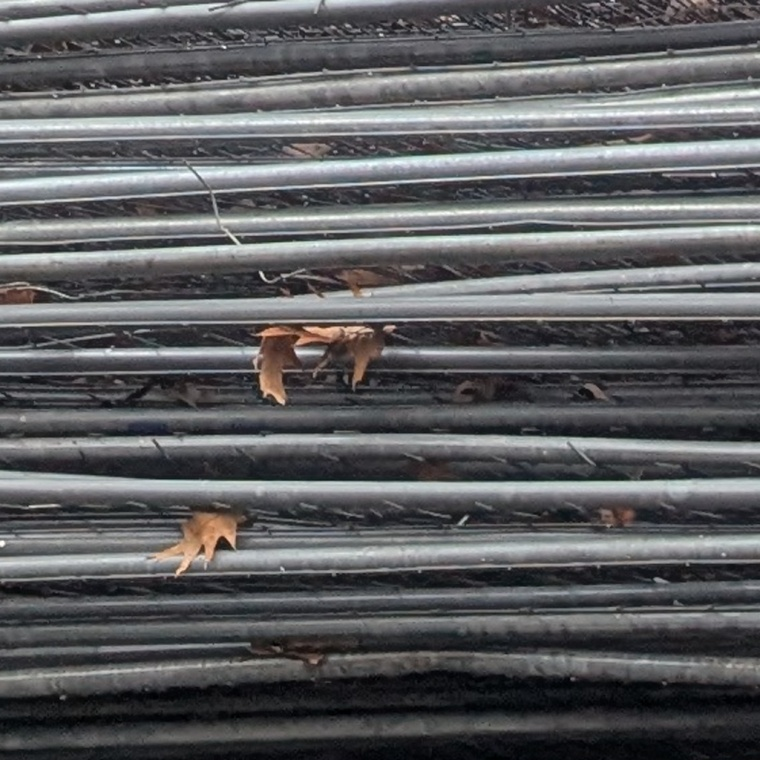
\includegraphics[width=0.205\textwidth]{abbildungen/stufe_T1_hintergrund.jpg} &
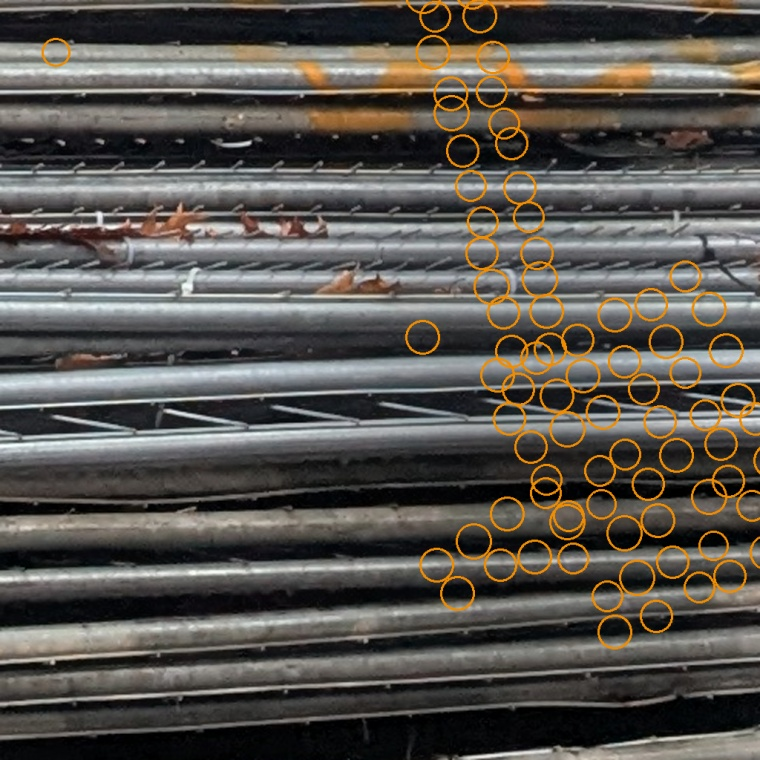
\includegraphics[width=0.205\textwidth]{abbildungen/stufe_T4_layout.jpg} &
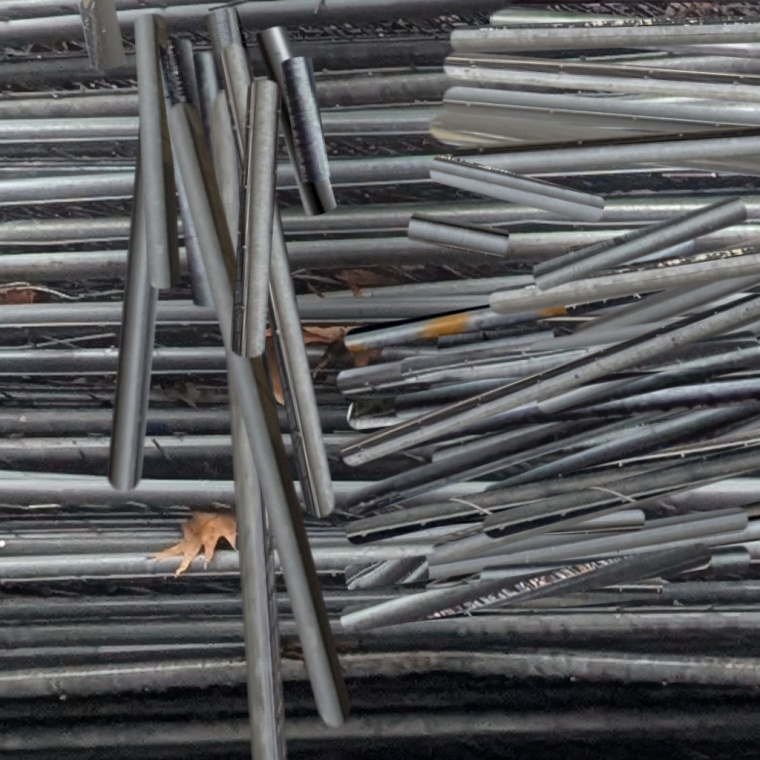
\includegraphics[width=0.205\textwidth]{abbildungen/stufe_T5_schaft.jpg} &
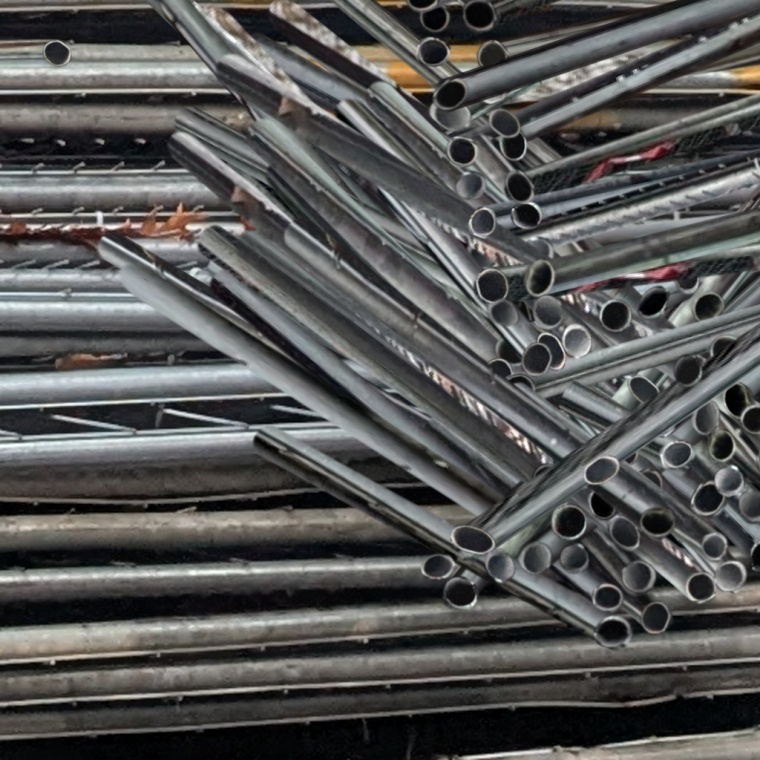
\includegraphics[width=0.205\textwidth]{abbildungen/stufe_T2T3_instanzen.jpg} \\[0.2em]
{\small\textbf{T1} Hintergrund} & {\small\textbf{T4} Layout} &
{\small\textbf{T5} Rohrschaft} & {\small\textbf{T2/T3} Instanzen} \\
\end{tabular}
\end{center}
\fuss{Zur Lesbarkeit ein Bild am oberen Ende des Größenbereichs --
Basisdurchmesser 44\px{} statt des Medians 22{,}5\px.}
\end{frame}

\note{%
\textbf{Folie 19 -- 0:30}\\
An den Bildern entlang, aber schnell -- sie tragen sich selbst.

T1: der gewählte Clean Plate nach Zoom, Ausschnitt und Spiegelung.
T4: die gezogenen Objektzentren des Layoutmodells -- ein gescherte Gitter, ein
bis drei Cluster, mit Rauschen auf jeder Gitterlage. Ohne dieses Rauschen
entstünden sichtbar künstliche Reihen, also selbst ein Merkmal.
T5: die Rohrschäfte, in paralleler Richtung, zu 75\,\% ganz hinten gemalt.
T2/T3: die Stirnflächen mit Instanzgeometrie und Photometrie.

Die Fußzeile ehrlich mitsprechen -- das hier ist kein typisches Bild, sondern
ein gut lesbares. Typische Bilder sehen unauffälliger aus, Zusatzfolie.}


\begin{frame}{Kein Generator darf Labels blind vergeben}
\vspace{-0.3em}
\begin{center}
{\large $\displaystyle \alpha_i^{\text{sichtbar}} = \alpha_i \prod_{j>i}\big(1-\alpha_j\big),
 \qquad v_i = \frac{\sum \alpha_i^{\text{sichtbar}}}{\sum \alpha_i}$}
\end{center}
\vspace{0.2em}
\grosszahl{20{,}1\,\%}{der gerenderten Instanzen bekommen \emph{kein}
Label}{34\,875 von 173\,100 -- verworfen, nicht vergessen}
\end{frame}

\note{%
\textbf{Folie 20 -- 0:35}\\
Inhaltlich der stärkste Teil der Pipeline. Ein zu 95\,\% verdecktes Objekt hat
kein sinnvolles Label -- also wird für \emph{jede} Instanz die Sichtbarkeit
\textbf{exakt} gerechnet, nach der Alpha-Kompositionsregel von Porter und
Duff. Die Buchhaltung läuft über die beschnittenen Alphafenster in
Malreihenfolge; das ist exakt und nicht approximiert.

Drei Verwerfungsregeln, dieselben, nach denen \code{val} und \code{test}
annotiert wurden -- das ist Anforderung A5: Sichtbarkeit unter 30\,\%
(30\,801 Objekte), weniger als 15\,\% der Fläche im Bild (3\,846), sichtbare
Box unter 5\px{} (228).

\textbf{Der Satz, auf den es ankommt:} Diese 20,1\,\% sind kein Verlust,
sondern der \emph{Ertrag} der Stufe. Sie markieren genau jene Bildstellen, an
denen ein naiver Generator ein \emph{falsches} Label gesetzt hätte -- und
\emph{kein} Label macht dieselbe Stelle zum korrekten harten Negativ.

Warum 30\,\%: Darunter wäre das Objekt auch für einen menschlichen Annotator
nicht mehr sicher identifizierbar.}


\begin{frame}{Der Nachweis ist nicht der optische Eindruck}{Erzeugte gegen gemessene Statistik}
\begin{center}\normalsize
\begin{tabular}{@{}lccc@{}}
\toprule
 & \textbf{real \code{val}} & \textbf{real \code{test}} &
   \textbf{synth.} \\
\midrule
Nachbarabstand (Median) & 1{,}11 & 1{,}26 &
  \textcolor{gut}{\textbf{1{,}17}} \\
Objekt-\Oe{} (Median, px) & 26{,}8 & 17{,}0 &
  \textcolor{gut}{\textbf{23{,}5}} \\
Nachbarn in $5\,\Oe$ & 10 & 10 & \textcolor{warn}{\textbf{13}} \\
\bottomrule
\end{tabular}
\end{center}
\fuss{Liegt \emph{zwischen} den beiden realen.
\textcolor{warn}{Bewusst abweichend:} dichtere Cluster als
Robustheitsreserve.}
\end{frame}

\note{%
\textbf{Folie 21 -- 0:35}\\
Die Botschaft: Ich behaupte \emph{nicht}, dass die Bilder \enquote{echt
aussehen}. Ich zeige, dass die \textbf{Statistik} stimmt -- gemessen über 1500
erzeugte Bilder mit 34\,027 Labeln.

Die Abweichung bei der Nachbarzahl selbst ansprechen, bevor gefragt wird:
13 statt 10 innerhalb von fünf Objektdurchmessern, im Maximum 61 statt 20.
Mehr Dichte im Training ist Reserve, weniger Dichte wäre eine Lücke. Die
Richtung ist also die sichere.

Die vollständige Tabelle mit allen sechs Kenngrößen liegt im Anhang -- wenn
jemand fragt, warum gerade diese drei, sofort dorthin springen. Die Auswahl
ist eine Interpretationsentscheidung, und das gebe ich auch so zu.

\textbf{Was diese Tabelle nicht zeigt:} dass die Kalibrierung der
\emph{Detektionsgüte} nützt. Sie belegt Verteilungstreue, nicht Wirkung. Diese
Trennung hält die Bilanz am Ende aufrecht.}


\begin{frame}{Trainingsaufbau}
\begin{punkte}
  \item \code{yolo26s-p2}, 9{,}66\,M Parameter, COCO-vortrainiert
  \item \textbf{P2-Kopf}: Zuweisungsgrenze 11{,}3 $\rightarrow$
        \textbf{5{,}7}\px{} -- unter alle Objektgrößen
  \item Modellauswahl auf dem \textbf{realen} \code{val};
        \code{test} berührt nichts
\end{punkte}
\fuss{Die Modellwahl ist \emph{keine} Variable der Experimente, sondern ihre
\textbf{Konstante}: Eine Ablation der Datenerzeugung soll auf dem Modell
laufen, das man auch einsetzen würde -- sonst kompensiert ein Datengewinn nur
die Schwäche eines unterlegenen Detektors.}
\end{frame}

\note{%
\textbf{Folie 22 -- 0:30}\\
Kurz halten. Die Fußzeile ist die eigentliche Aussage und die Antwort auf
\enquote{warum haben Sie die Architektur nicht abliert}.

Größe \enquote{s} folgt aus der Datenlage: eine Klasse, neun zugrunde liegende
Objektinstanzen, kleine Formvielfalt. Mehr Kapazität könnte die synthetischen
Eigenheiten nur memorieren.

Der P2-Kopf senkt die Schrittweite der feinsten Detektionsebene von 8 auf 4
und kostet dabei \emph{keine} Parameter -- er hat 2,9\,\% weniger als das
Basismodell -- sondern Speicher.

\code{imgsz}=1024 ist gleich der Leinwandgröße des Generators: Die
synthetischen Bilder durchlaufen \emph{keine} Skalierung, die kalibrierte
Größenverteilung bleibt exakt erhalten. Das ist A2.

Falls nach den zwei Budgets gefragt wird -- Referenz 6000 Bilder / 60 Epochen,
Ablation 3000 / 30 --: sie kommen auf den Ablationsfolien als Marker wieder.
Batch 8 statt 16 war erzwungen, nicht gewählt: die P2-Merkmalskarte belegt bei
Batch 16 rund 23,5\,GB, frei waren etwa 25.}


\trenner{Teil 4}{Das Ergebnis}

% ==========================================================================
\section{Ergebnis}
% ==========================================================================

\begin{frame}[plain]
\vfill
\zweizahl{\zrefValMap}{\code{val}}{\zrefTestMap}{\code{test}}
\begin{center}\Large \mAPfifty{} auf echten Aufnahmen\end{center}
\fuss{\hfill Trainiert auf \emph{null} handannotierten Bildern.
\code{test} berührt Training und Modellauswahl nie. \hfill}
\vfill
\end{frame}

\note{%
\textbf{Folie 24 -- 0:35 -- die Antwort auf die Aufgabenstellung}\\
Hier Zeit lassen. Das ist das Ergebnis, auf das Folie 5 hingearbeitet hat:
von null annotierten Trainingsbildern zu \zrefValMap{} und \zrefTestMap{}
\mAPfifty{} auf echten Aufnahmen.

Am $F_1$-optimalen Betriebspunkt: bestes $F_1$ \zrefValFf{} bzw.\
\zrefTestFf, Rückruf \zrefValRec{} / \zrefTestRec{} bei Precision
\zrefValPrec{} / \zrefTestPrec.

Konkret auf \code{test}: \znPredTest{} Detektionen, davon \zfpTest{} nicht auf
einem annotierten Objekt, und \zfnTest{} der 89 Stirnflächen übersehen.

Wichtig für die Einordnung: \code{test} ist der \emph{schwierigere} der beiden
Splits -- kleinere Objekte (Median 17,0 gegen 26,8\px), lockerere Packung,
mehr angeschnittene Boxen -- und zugleich der, der Training und Modellauswahl
nie berührt hat.

Falls nach \mAPseven{} gefragt wird: kommt in Teil 6, das ist ein
Metrikbefund und keine Detektionsschwäche. Nicht vorziehen.}


\begin{frame}{Aufgabe gelernt -- oder Artefakte?}
\zweizahl{\zsimRealVal\,\%}{Abstand auf \code{val}}{\zsimRealTest\,\%}{Abstand
auf \code{test}}
\fuss{Sim-to-Real-Abstand: Differenz zum synthetischen Split. Bei reinem
Artefaktlernen wäre synthetisch nahezu perfekt und real katastrophal --
\textbf{genau dieses Muster tritt nicht auf}. Ein \emph{Indiz}, kein Beweis:
die Schranke von Ben-David nagelt die Divergenz nach \emph{unten} fest.}
\end{frame}

\note{%
\textbf{Folie 25 -- 0:35}\\
Methodisch die interessantere Zahl als das Ergebnis selbst. \code{sval} sind
400 synthetische Bilder derselben Pipeline mit anderem Seed; der Split trennt
zwei Fragen: \emph{Kann das Modell die Aufgabe überhaupt?} und
\emph{überträgt es sich auf echte Bilder?}

Die Gegenprobe laut rechnen, sie macht die Größenordnung deutlich: Hätte das
Netz die Einfügeartefakte gelernt, wäre der synthetische Fehler bei etwa
0,005 und der reale bei 0,95; die Ben-David-Schranke ergäbe
$\tfrac12\, d + \lambda \geq 0{,}94$. Gemessen sind \zepsDiff{}.

\textbf{Die Redlichkeit gehört auf diese Folie und in den Satz:} Die
Ungleichung nagelt die Summe nach \emph{unten} fest. Dass die Divergenz klein
\emph{ist}, kann sie nicht belegen -- sie zeigt nur, dass die Daten eine große
nicht erzwingen. Deshalb bleibt es ein Indiz, und deshalb steht es in der
Bilanz unter \enquote{indirekt gestützt} und nicht unter \enquote{belegt}.

Das ist zugleich der einzige \emph{direkte} empirische Hinweis darauf, dass
die Anti-Abkürzungs-Maßnahmen S1--S6 überhaupt greifen.}


\begin{frame}{Eine Vorhersage aus Kapitel 3}
\vfill
\begin{center}
{\large $\displaystyle d_{\text{eff}} = d \cdot \frac{M}{N}$}
\end{center}
\vfill
\begin{center}\large
Bei \code{imgsz}~640 schrumpfen die 12--36\px{}\\
des 2459\px{} breiten Bildes auf \textbf{3--9\px}.
\end{center}
\vfill
\fuss{Die Schrittweite der feinsten Standard-Detektionsebene ist 8\px.
Diese Rechnung stand \emph{vor} den Läufen.}
\end{frame}

\note{%
\textbf{Folie 26 -- 0:30}\\
Diese Folie ist bewusst \emph{vor} der Messung. Der Punkt ist nicht die
Formel, sondern die Reihenfolge: Die Rechnung stand in Kapitel 3, bevor
gemessen wurde. Eine eingetroffene Vorhersage ist methodisch mehr wert als
ein nachträglich erklärter Effekt -- das sage ich hier ausdrücklich, weil die
nächsten zwei Folien sonst wie eine Entdeckung wirken.

Detektoren verarbeiten Bilder in fester Netzeingangsgröße $M$; ein Bild mit
längster Kante $N$ wird um $M/N$ skaliert. Für $N = 2459$, $d = 27$\px{} und
$M = 640$ ergibt das 7,0\px{} -- weniger als die Schrittweite 8 der feinsten
Standardebene.

Falls nach der Zuweisungsgrenze $S\sqrt2$ gefragt wird: Zusatzfolie. Kurzform
-- ein ankerfreier Kopf weist einer Position genau dann ein Objekt zu, wenn
ihr Zentrum darin liegt; unterhalb von $S\sqrt2 = 11{,}3$\px{} hängt das von
der Lage im Gitter ab.}


\begin{frame}{Und so sieht sie gemessen aus}
\bild{abbildungen/neu_imgsz.png}
\fuss{Zehn Auflösungen, kein Neutraining. Gewählt: \code{imgsz}
\zbestImgsz{} nach \mAPall{} auf \code{val}.}
\end{frame}

\note{%
\textbf{Folie 27 -- 0:30}\\
Der Verlauf ist auf beiden Splits derselbe: steiler Anstieg bis etwa 1300\px,
danach ein flaches Optimum.

Der Rückruf bricht bei 640 auf \zswValNiedrigRec{} ein -- das Modell
\emph{findet} die Objekte nicht mehr, es lokalisiert sie nicht bloß
schlechter. Das ist der Unterschied, auf den es ankommt.

\textbf{Das Optimum liegt, wo die effektive Objektgröße zum Trainingsmedian
passt} (23,5\px): auf \code{val} bei \zswValBestAt{} mit
\zswValBestDeff\px{} im Netzeingang, auf \code{test} bei \zswTestBestAt{} mit
\zswTestBestDeff\px. Der Effekt ist in \emph{beide} Richtungen sichtbar --
auch zu große Auflösung kostet.

Sauberkeit der Auswahl, falls gefragt: Eine Wahl je Split wäre
Hyperparameterselektion auf dem Testsatz und würde dessen Zahlen wertlos
machen. Deshalb ein Wert für beide.

Nebenbefunde nur bei Nachfrage: TTA ist bei diesem Modell nicht verfügbar,
NMS greift nicht, weil YOLO26 NMS-frei arbeitet.}


\begin{frame}{Der größte gemessene Einzeleffekt der Arbeit}
\sprungzahl{}{\zswValNiedrig}{\zswValBest}{$+\,\zswValGain\PP$ \mAPfifty{}
auf \code{val}}{\code{imgsz} 640 $\rightarrow$ \zswValBestAt{} -- mehr als
\emph{alle} Augmentierungsentscheidungen zusammen}
\fuss{\textbf{Und es ist keine Augmentierungsentscheidung.} Die
Auflösungsfrage gehört \emph{zuerst} geklärt.}
\end{frame}

\note{%
\textbf{Folie 28 -- 0:35 -- die unbequeme Bilanz}\\
\textbf{Der Satz aus der Fußzeile muss gesprochen werden}, sonst dreht sich
die Aussage: Isoliert liest sich diese Zahl wie ein Erfolg der Arbeit. Sie ist
aber das Gegenargument gegen ihren eigenen Aufwand.

\zswValGain\PP{} zwischen 640 und dem Optimum. Alle
Augmentierungsentscheidungen zusammen bewegen sich in der Größenordnung
weniger Prozentpunkte.

Das relativiert die Pipeline \emph{nicht} -- ohne sie gäbe es überhaupt keinen
Trainingsdatensatz -- aber es verschiebt die Priorität. Diese Unbequemlichkeit
selbst aussprechen; sie steht auch so in der Diskussion der Arbeit.

Was hier trägt: Eine einzige Kenngröße, die effektive Objektgröße relativ zur
Schrittweite, begründet fünf unabhängige Entscheidungen -- Kalibrierung des
Generators, Trainingsauflösung, P2-Kopf, Inferenzauflösung -- und erklärt
diesen Effekt. Das ist das methodisch belastbarste Ergebnis der Arbeit.}


\trenner{Teil 5}{Die Prüfung}

% ==========================================================================
\section{Prüfung}
% ==========================================================================

\begin{frame}[plain]
\botschaft{Die Pipeline schneidet ihre Verdecker aus \textbf{echten}
Aufnahmen.\\[0.7em]
Begründung: ein \emph{gemalter} Balken hätte eine andere Textur-, Rausch- und
Glanzstatistik.\\[0.7em]
{\Large\color{warn}Das ist ein Argument. Keine Messung.}}
\end{frame}

\note{%
\textbf{Folie 30 -- 0:35}\\
Jetzt wird die Behauptung von Folie 15 eingelöst. Erst begründen, warum
\emph{diese} Frage geprüft wird und keine andere:

An der Okklusionsstufe sind zwei Fragen zu stellen -- \emph{wie viel} verdeckt
wird und \emph{woraus} die Verdecker bestehen. Die erste ist keine
Entwurfsfreiheit: In den Realbildern liegen ausnahmslos Rohre vor den
Stirnflächen, das ist physikalische Randbedingung. Frei entschieden ist nur
die zweite.

Und die ist \textbf{teuer}: eine eigene Verarbeitungsstufe mit
Struktur-Tensor, Achsdetektion und Plausibilitätsprüfung -- plus die Bindung
an die vier vorhandenen Clean Plates. Ein prozedural gezeichneter Balken wäre
in zwanzig Zeilen Code geschrieben und in beliebiger Zahl verfügbar.

Der letzte Satz der Folie ist der Grund für das Experiment. Die
Begründungspflicht von Folie 8 hat genau diese eine Stelle sichtbar
gemacht.}


\begin{frame}{Drei Bibliotheken, eine Leiter}
\budgetmarker
\bild{abbildungen/neu_balken.png}
\fuss{\hfill \textbf{B0} photographisch \;$\rightarrow$\;
\textbf{B1} prozedural, kalibriert \;$\rightarrow$\;
\textcolor{warn}{\textbf{B2} flächig grau} \hfill}
\end{frame}

\note{%
\textbf{Folie 31 -- 0:35}\\
Die drei Arme:
\begin{itemize}
  \item \textbf{B0}: die 56 aus den Clean Plates geschnittenen Stangen -- die
        Bibliothek der Pipeline, also der Kontrollarm.
  \item \textbf{B1}: ein Zylindermodell aus Lambert-Term, Glanzlicht,
        Umgebungslicht, Längsvariation und Korn, an B0 kalibriert: Grauwert,
        Kornstärke, Farbsättigung, Längsvariation und Querschnittskontrast
        treffen die gemessenen Werte.
  \item \textbf{B2}: konstantes Grau in derselben Maske. Kein Verlauf, kein
        Glanzlicht, kein Korn, keine Farbe -- der \enquote{gezeichnete
        Balken}, vor dem die Pipeline warnt.
\end{itemize}

\textbf{Warum eine Leiter und kein Zweiervergleich:} \enquote{Echt gegen
gezeichnet} könnte nur sagen, \emph{dass} ein Unterschied besteht -- es wären
viele Faktoren gleichzeitig verändert. Die Leiter sagt zusätzlich, \emph{wie
weit} ein prozedurales Modell trägt, und trennt damit \emph{Herkunft} von
\emph{Statistik}. Das ist der eigentliche Entwurf des Versuchs.

Fairness von B1 selbst nennen: B1 ist \emph{ein} sorgfältig kalibriertes
Modell, nicht das bestmögliche. Kalibriert sind fünf \textbf{skalare}
Kennwerte; nicht getroffen ist die räumliche Korrelation des Restsignals --
das Korn von B1 ist weißes Rauschen, das von B0 enthält Kratzer, Rost und
JPEG-Blockstruktur.}


\begin{frame}{Dieselbe Szene, drei Bibliotheken}
\budgetmarker
\bild{abbildungen/neu_balken_szene.png}
\fuss{Horizontal = Hintergrund, diagonal = eingefügt.
\textcolor{gut}{Grün} die Labels -- in allen drei Armen dieselben.}
\end{frame}

\note{%
\textbf{Folie 32 -- 0:25}\\
Die drei Bilder anschauen lassen, wenig sagen:

In B0 sind eingefügte und Hintergrund-Rohre nicht zu unterscheiden -- sie
stammen aus derselben Aufnahme. In B1 wirken die eingefügten glatter, bleiben
aber plausible Zylinder. In B2 sind sie als flache graue Balken sofort
erkennbar. \emph{Genau das} ist die Abkürzung, deren Kosten gemessen werden.

Die grünen Labels sind der Übergang zur nächsten Folie: Sie sind in allen drei
Armen exakt dieselben. Das ist kein Zufall, sondern konstruiert.}


\begin{frame}{Warum der Versuch \emph{gepaart} ist}
\budgetmarker
\kasten{\Large Die Labelverzeichnisse aller drei Arme sind\\[0.25em]
{\color{akzent}\bfseries byte-identisch}\\[0.2em]
{\footnotesize SHA-256: \code{951f6e23e65486f1}}}
\vspace{0.6em}
\begin{center}\large
Es bleibt genau \textbf{eine} Variable:
die RGB-Werte in den Masken.
\end{center}
\end{frame}

\note{%
\textbf{Folie 33 -- 0:35}\\
Hier wird der Versuchsaufbau gewonnen. Ruhig Zeit lassen, das ist die
methodisch stärkste Folie des Vortrags.

Wie es zustande kommt: Jede prozedurale Stange übernimmt von ihrem
photographischen Gegenstück die exakte Pixelgröße und die exakte Alphamaske.
Der Generator zieht seine Stange über \code{rng.integers(0,~56)} -- also ist
die Zufallsfolge in allen drei Läufen identisch, und weil die Alphamasken
identisch sind, ist es auch die Sichtbarkeitsrechnung.

Nachprüfbar: Labelzahl 68\,281, mittlere Sichtbarkeit 0,901, Anteil
teilverdeckter Objekte 29,9\,\% -- in allen drei Armen exakt gleich. Der
SHA-256 der drei Labelverzeichnisse ist derselbe, die Bildverzeichnisse sind
paarweise verschieden.

\textbf{Warum das zählt:} Eine gewöhnliche Datensatz-Ablation muss
offenlassen, ob ein Ergebnisunterschied von einer anderen Objektverteilung,
einer anderen Labelzahl oder einem anderen Verdeckungsgrad herrührt. Hier
nicht. Es gibt keine zweite Variable, auf die man einen Unterschied schieben
könnte.}


\begin{frame}{Das Ergebnis}
\budgetmarker
\begin{center}\normalsize
\begin{tabular}{@{}lcccc@{}}
\toprule
 & \multicolumn{2}{c}{\code{test}} & \multicolumn{2}{c}{\code{val}} \\
 & \mAPfifty{} & Rückruf & \mAPfifty{} & $F_1$ \\
\midrule
B0 photographisch & \zBZeroTestMap{} & \textbf{\zBZeroTestRec} &
  \textbf{\zBZeroValMap} & \textbf{\zBZeroValFf} \\
B1 prozedural & \textbf{\zBOneTestMap} & \zBOneTestRec{} &
  \zBOneValMap{} & \zBOneValFf{} \\
\textcolor{warn}{B2 flächig grau} & \textcolor{warn}{\zBTwoTestMap} &
  \textcolor{warn}{\zBTwoTestRec} & \zBTwoValMap{} & \zBTwoValFf{} \\
\bottomrule
\end{tabular}
\end{center}
\fuss{Belastbar ist nicht die Einzeldifferenz, sondern die
\textbf{Konsistenz}: dieselbe Richtung über drei Arme, vier Metriken und
zwei Splits. Bootstrap $\pm\zbootTestStd$.}
\end{frame}

\note{%
\textbf{Folie 34 -- 0:40}\\
Diese Tabelle bleibt im Hauptteil, obwohl sie die dichteste Folie ist -- weil
die \emph{Nebeneinanderstellung} das Argument ist. Drei Befunde, in dieser
Reihenfolge:

\textbf{(1) Der naive Balken kostet messbar.} Auf dem unberührten \code{test}
gegenüber B0: $-\zablBTestGap\PP$ \mAPfifty, $-\zablBTestGapFf\PP$ $F_1$,
$-\zablBTestGapRec\PP$ Rückruf. Die Zählung fällt von \zBZeroTestCnt{} auf
\zBTwoTestCnt{} von 89 Objekten. Das ist der größte Effekt, den diese Arbeit
über einen Eingriff in die \emph{Trainingsdaten} gemessen hat -- mehr als das
Doppelte des Bootstrap-Intervalls.

\textbf{(2) Photographisch muss er nicht sein.} B1 ist auf \code{test} von B0
nicht zu unterscheiden, $F_1$ sogar leicht höher; auf \code{val} liegt es
$\zablBValGapEins\PP$ darunter. \textbf{Die Splits widersprechen sich in der
Richtung -- die Differenz ist nicht entscheidbar.} Das ist eine
\textbf{Nicht-Ablehnung}, kein Nachweis der Gleichheit. Diesen Satz genau so
sagen.

\textbf{(3) Die Konsistenz trägt, nicht die Einzeldifferenz.} Die Reihenfolge
B0 $>$ B1 $>$ B2 ist in drei der vier Zellen aus Größenklasse $\times$ Split
monoton, und die Zahl der Falsch-Negativen widerspricht ihr in keinem Fall.

Auf den Budgetmarker zeigen, falls jemand \zBZeroTestMap{} gegen die
\zrefTestMap{} von Folie 24 stellt.}


\begin{frame}{Der Verlust sitzt dort, wo verdeckt wird}
\budgetmarker
\sprungzahl{}{\zBZeroTestRecKlein}{\zBTwoTestRecKlein}{Rückruf auf dem
kleinsten Objektdrittel von \code{test}}{$-23\PP$ -- gegen nur $3{,}4\PP$
bei den größeren zwei Dritteln}
\fuss{Kleine Stirnflächen liegen tief im Stapel -- dort kreuzen die Rohre
einander.}
\end{frame}

\note{%
\textbf{Folie 35 -- 0:35}\\
Das ist der Befund, der die Deutung erzwingt. Auf dem kleinsten Drittel von
\code{test} -- Objekte bis \zgrenzeTest\px, \znKleinTest{} Stück -- fällt der
Rückruf von \zBZeroTestRecKlein{} über \zBOneTestRecKlein{} auf
\zBTwoTestRecKlein.

23 Prozentpunkte gegen 3,4 bei den größeren zwei Dritteln. Der Verlust ist
also nicht diffus, er ist \emph{lokalisiert}.

Und er sitzt genau dort, wo man ihn erwarten würde -- das ist das Argument der
Fußzeile. Kleine Stirnflächen liegen tief im Stapel, dort kreuzen die Rohre
einander, und genau diese Situation kennt B2 aus dem Training nicht.

Einschränkung, die dazugehört: Die Aufschlüsselung nach Objektgröße ist ein
\emph{Stellvertreter} für die Stapeltiefe. Die realen Bilder tragen keine
Verdeckungsannotation, der Verdeckungsgrad je Objekt ist also nicht direkt
messbar. Sagen, wenn gefragt wird.}


\begin{frame}{Aber anders als erwartet}
\budgetmarker
\begin{center}\large
Die Precision bleibt \textbf{unberührt}:
\; \zBTwoTestPrec{} (B2) gegen \zBZeroTestPrec{} (B0)
\end{center}
\vspace{0.6em}
\kasten{\Large Keine Abkürzung, sondern eine\\[0.3em]
{\color{akzent}\bfseries Domänenlücke beim Verdecker}}
\end{frame}

\note{%
\textbf{Folie 36 -- 0:35 -- der intellektuelle Kern}\\
Hier fällt der Befund \emph{anders} aus als vorhergesagt, und das ist die
lehrreiche Stelle. Offen als Verfehlung der eigenen Erwartung darstellen.

Kapitel 3 hatte eine \textbf{Abkürzung} erwartet: Das Netz lernt \enquote{hier
endet ein künstlicher Balken} und produziert außerhalb der Trainingsverteilung
Falschpositive. Gemessen wird das Gegenteil -- die Precision bleibt
unberührt, es bricht ausschließlich der Rückruf ein.

Also ist es keine Abkürzung im engeren Sinn, sondern eine gewöhnliche
\textbf{Domänenlücke} -- nur eben eine, die nicht das Objekt betrifft, sondern
das, was davorliegt.

\textbf{Konsequenz, die man ziehen muss:} Die Signaturenliste S1--S6
beschreibt für Okkluder nicht das richtige Versagensmuster. Sie hat auf die
richtige \emph{Größe} gezeigt -- die Textur- und Rauschstatistik des
Verdeckers -- aber das falsche Fehlerbild vorhergesagt. Das gehört gesagt,
nicht kaschiert.}


\begin{frame}[plain]
\botschaft{Nicht die \textbf{Herkunft} der eingefügten Pixel entscheidet,
sondern ob ihre \textbf{Statistik} zur Umgebung passt.\\[0.8em]
{\Large Wer Copy-Paste-Synthese betreibt, muss die Realismusanforderungen an
das Objekt auch an alles stellen, was \emph{davor} liegt.}}
\end{frame}

\note{%
\textbf{Folie 37 -- 0:35 -- Kernsatz 2 von 3, der Beitrag der Arbeit}\\
Wenn nur ein Satz hängen bleiben soll, dann dieser. Langsam, und danach eine
Pause.

Die Behauptung der Pipeline ist damit \textbf{in der Sache bestätigt und in
ihrer starken Form widerlegt}:
\begin{itemize}
  \item \emph{Bestätigt:} Die Textur- und Rauschstatistik des Verdeckers ist
        eine relevante Größe, kein Detail -- \zablBTestGap\PP{} \mAPfifty{}
        für einen flächig grauen Balken.
  \item \emph{Widerlegt in der starken Form:} Photographisch muss er nicht
        sein. Die aufwendigste Vorstufe -- Struktur-Tensor, Achsdetektion,
        Bindung an vier Clean Plates -- lässt sich durch rund vierzig Zeilen
        Beleuchtungsmodell ersetzen, an fünf messbaren Kennwerten kalibriert.
\end{itemize}
Was \emph{nicht} entfallen darf, ist die Kalibrierung: Der Unterschied
zwischen B1 und B2 ist allein die Frage, ob der Balken Schattierung,
Glanzlicht, Korn und Farbstich der Umgebung trägt.

Und wo photographisches Material fehlt, ist ein kalibriertes Modell damit die
gleichwertige Alternative -- das ist die übertragbare Aussage.}


\trenner{Teil 6}{Das Messinstrument}

% ==========================================================================
\section{Metrik}
% ==========================================================================

\begin{frame}{Ein Wert, der nicht passt}
\begin{center}\normalsize
\begin{tabular}{@{}lcc@{}}
\toprule
 & \mAPfifty{} & \mAPseven{} \\
\midrule
\code{test} & \zrefTestMap{} & \textcolor{warn}{\textbf{\zrefTestMapS}} \\
\bottomrule
\end{tabular}
\end{center}
\vspace{0.5em}
\begin{center}\large
Das Modell \emph{findet} jedes Objekt -- und trifft\\
die Boxgröße systematisch zu klein.
\end{center}
\fuss{Auf dem \emph{synthetischen} Split stimmt sie auf wenige Promille
(\zboxSvalRatio) -- die Boxregression funktioniert.}
\end{frame}

\note{%
\textbf{Folie 39 -- 0:35}\\
Das ist der Wert, den eine Kommission ohnehin gesehen hat. Ihn selbst
aufgreifen, nicht darauf warten.

Die Beweiskette in drei Schritten, und die Reihenfolge ist der Beweis:
\begin{enumerate}
  \item Auf \code{sval} trifft das Modell die Boxgröße exakt --
        Verhältnis \zboxSvalRatio, Abweichung \zboxSvalOff\px. Die Regression
        funktioniert.
  \item Auf den Realbildern liegt sie 10\,\% darunter (\zboxTestRatio{} auf
        \code{test}, \zboxValRatio{} auf \code{val}), der
        \emph{Zentrums}versatz bleibt aber mit \zboxTestCtr{}
        Objektdurchmessern im Bereich der Annotationsgenauigkeit. Es ist also
        ein \textbf{Größen}fehler, kein Positionsfehler.
  \item Also liegt die Ursache nicht im Modell, sondern in der
        \textbf{Labelkonvention}: Die Generatorboxen folgen der
        $\alpha > 0{,}5$-Kontur der Alphamaske, die Handannotation umschließt
        das Objekt großzügiger.
\end{enumerate}
Damit ist Anforderung A5 nur \emph{annähernd} erfüllt -- der Restversatz
beträgt messbar \zboxValOff{} bis \zboxTestOff\px. Das gebe ich so zu.}


\begin{frame}{Am Modell nichts geändert}
\sprungzahl{}{\zsensTestMapSOrig}{\zsensTestMapSNeu}{\mAPseven{} auf
\code{test}}{alle Boxen um \zsensTestGrow\px{} je Seite aufgeweitet, neu
ausgewertet}
\fuss{\mAPfifty{} und $F_1$ bleiben davon \textbf{unberührt} --
\mAPfifty{} fällt sogar leicht. Die Aufteilung ist damit eindeutig:
\mAPseven{} und \mAPall{} messen hier zu einem erheblichen Teil eine
Konventionsdifferenz, nicht die Detektionsgüte.}
\end{frame}

\note{%
\textbf{Folie 40 -- 0:35}\\
Die Sensitivitätsrechnung: alle vorhergesagten Boxen um den gemessenen
medianen Fehlbetrag von \zsensTestGrow\px{} je Seite aufweiten und neu
auswerten. Am Modell wird nichts geändert.

\mAPseven{} steigt von \zsensTestMapSOrig{} auf \zsensTestMapSNeu, \mAPall{}
von \zsensTestMapAOrig{} auf \zsensTestMapANeu{} -- während \mAPfifty{} von
\zsensTestMapOrig{} auf \zsensTestMapNeu{} leicht \emph{fällt} und das $F_1$
mit \zsensTestFfNeu{} unverändert bleibt.

\textbf{Wichtig für die Fairness:} Das \emph{rechtfertigt} \mAPfifty{} als
Leitgröße nachträglich -- aber die Festlegung stand vorher, in Abschnitt 7.1,
und stützt sich auf die IoU-Empfindlichkeit bei Kleinobjekten. Ich habe nicht
nachträglich die Metrik gewählt, die besser aussieht.

Und noch ein Punkt: Der Versatz trägt \emph{nichts} zur Ben-David-Schranke
bei, weil das Aufweiten \mAPfifty{} nicht verbessert. Bei der
Zuordnungsschwelle 0,5 ist die Konventionsdifferenz wirkungslos.

Falls gefragt wird, ob das ein Fehler der Arbeit sei: Ja -- und es ist
gleichzeitig der billigste offene Gewinn. Eine geänderte Boxschwelle im
Generator, rund \zsensTestGain{} Punkte \mAPseven.}


\begin{frame}[plain]
\botschaft{Bei programmatisch erzeugten Labels wird die
\textbf{Labelkonvention} selbst zu einer messbaren Größe.\\[0.8em]
{\Large Wer Lokalisierungsmetriken bei 20\px-Objekten berichtet, muss sie
zuerst kennen.}}
\end{frame}

\note{%
\textbf{Folie 41 -- 0:20 -- Kernsatz 3 von 3}\\
Kurz und ohne Zusatz. Der Beleg liegt eine Folie zurück, die Reihenfolge muss
sitzen.

Das ist ein Ergebnis für sich, nicht nur eine Fehlerdiagnose: Zwei Pixel
Konventionsdifferenz verschieben \mAPseven{} um mehr als vierzig Punkte, ohne
dass sich am Modell etwas ändert. Wer das nicht kennt, interpretiert
Lokalisierungsmetriken bei Kleinobjekten falsch.}


\trenner{Teil 7}{Bilanz}

% ==========================================================================
\section{Bilanz}
% ==========================================================================

\begin{frame}{Was ist belegt, was ist nur begründet?}
\grosszahl{1 von 43}{Parameterwerten ist kontrolliert
\textbf{abliert}}{Das ist wenig, und es soll nicht schöngeredet werden}
\fuss{Die Begründungssystematik trägt den \emph{Entwurf}. Der experimentelle
Nachweis trägt genau \emph{einen Punkt} daraus.}
\end{frame}

\note{%
\textbf{Folie 43 -- 0:35}\\
Diese Folie \textbf{nicht} überspringen, auch wenn die Zeit knapp wird. Sie
ist der Grund, warum die Arbeit als redlich gelesen werden kann.

Den Satz selbst aussprechen, ohne Beschönigung. Dann die Begründung
nachliefern -- warum \emph{gerade} dieser eine:
\begin{itemize}
  \item Es war die \textbf{teuerste} Einzelentscheidung der Pipeline.
  \item Sie war ausschließlich durch ein \textbf{Argument} gedeckt, nicht
        durch eine Messung.
  \item Sie ließ sich als \textbf{gepaarter} Versuch anlegen --
        byte-identische Labels, keine zweite Variable. Diesen Vorzug hat kaum
        eine Datensatz-Ablation.
\end{itemize}
Die fünf Belegstände der Arbeit, falls nachgefragt wird: \emph{abliert}
(Herkunft der Okkluder), \emph{gemessen ohne Neutraining}
(Inferenzauflösung), \emph{kalibriert an der Verteilung} (Größenbereich,
Gitterabstände), \emph{indirekt gestützt} (das Bündel S1--S6 über den
Sim-to-Real-Abstand) und \emph{begründet, nicht belegt} (Matting-Schwelle,
Farb-, Unschärfe- und Rauschangleich, JPEG, Schlagschatten). Die vollständige
Tabelle ist eine Zusatzfolie.

Wer fragt \enquote{warum nicht mehr Ablationen}: Rechenzeit -- und die Arme
zum Verdeckungs\emph{grad} liegen trainiert vor, Zusatzfolie Ablation A.}


\begin{frame}{Grenzen}{Die schwerste liegt in der Bewertung, nicht in der Pipeline}
\begin{punkte}
  \item \textbf{Je \emph{ein} Bild pro Split}
  \item \textbf{Je ein Lauf pro Arm}
  \item \textbf{Nur diffuses Licht} im Quellmaterial
\end{punkte}
\fuss{Bootstrap $\pm\zbootValStd$ / $\pm\zbootTestStd$; belastbar sind die
\code{test}-Zahlen.}
\end{frame}

\note{%
\textbf{Folie 44 -- 0:35}\\
Je Punkt ein Satz, nicht mehr:
\begin{itemize}
  \item \textbf{Ein Bild pro Split} ist die schwerwiegendste methodische
        Schwäche der Arbeit, und ich nenne sie zuerst. Unterschiede unter dem
        Bootstrap-Intervall sind nicht entscheidbar -- deshalb argumentiert
        die Ablation über Konsistenz und nicht über Einzeldifferenzen.
  \item \textbf{Ein Lauf pro Arm} ist die gewichtigste Einschränkung der
        Ablation -- und die einzige, die reine Rechenzeit behebt: drei Seeds
        je Arm wären neun statt drei Läufen.
  \item \textbf{Nur diffuses Licht}: Die Fehleranalyse weist \enquote{Enden
        ohne sichtbaren hellen Kranz} als den Fehlertyp aus, der \emph{nicht}
        auf Objektgröße zurückgeht. Das ist genau diese Lücke.
\end{itemize}
Weitere Grenzen, falls gefragt: neun Quellobjekte (jedes erscheint rund
15\,100-mal), Reflect-Padding erzeugt Spiegelsymmetrie -- die Maßnahme gegen
S1 erzeugt also eine schwächere neue Auffälligkeit --, und die Schaftrichtung
ist am Cluster kalibriert, nicht am Hintergrund.

Das ist der bessere Ort für Selbstkritik als die Diskussion: Was ich selbst
benenne, kann mir nicht vorgehalten werden.}


\begin{frame}{Nächste Schritte}{Nach erwartetem Nutzen, nicht nach Aufwand}
\begin{punkte}
  \item \textbf{Labelkonvention angleichen}
        {\normalsize\color{grau}-- $\approx \zsensTestGain$ Punkte \mAPseven}
  \item \textbf{10--20 Realbilder, 3 Seeds je Arm}
  \item \textbf{Die übrigen S1--S6-Maßnahmen ablieren}
  \item \textbf{Quellmaterial bei harter Sonne und Nässe}
\end{punkte}
\end{frame}

\note{%
\textbf{Folie 45 -- 0:20}\\
Zügig, das ist eine Liste. Zwei Bemerkungen:

Punkt 1 ist der billigste große Gewinn der Liste und vor jeder weiteren
Optimierung zu erledigen -- eine geänderte Boxschwelle im Generator genügt.

Punkt 2 sind die beiden Dinge, die aus einem \emph{Hinweis} einen
\emph{Nachweis} machen. Solange sie fehlen, bleibt \enquote{B1 ist so gut wie
B0} eine Nicht-Ablehnung.

Zu Punkt 3: Diese Arbeit hat den Weg für \emph{eine} Maßnahme vorgemacht; je
ein Lauf mit abgeschaltetem Farb-, Rausch- und Unschärfeangleich sowie ohne
JPEG-Durchlauf würde die restlichen Signaturen entsprechend prüfen. Zielgröße
wäre der Sim-to-Real-Abstand.}


\begin{frame}{Drei Einsichten}
\begin{punkte}
  \item Bei rein synthetischen Daten ist die \textbf{Pipeline die Hypothese}
  \item Nicht die Herkunft der Pixel entscheidet, sondern ihre
        \textbf{Statistik}
  \item \textbf{Auflösung dominiert} -- und die Labelkonvention ist Teil des
        Messinstruments
\end{punkte}
\fuss{\hfill \mAPfifty{} \textbf{\zrefValMap} und \textbf{\zrefTestMap} auf
zwei echten Aufnahmen -- für eine Anwendung, für die \emph{kein einziges}
handannotiertes Trainingsbild existiert. \hfill}
\end{frame}

\note{%
\textbf{Folie 46 -- 0:35 -- Schluss}\\
Langsam. Das ist der letzte Eindruck, und die drei Punkte sind genau die drei
Kernsätze von den Folien 7, 37 und 41 -- also Wiedererkennung, keine neue
Information.

Zu jedem einen Satz:
\begin{enumerate}
  \item Jede Entscheidung über eine Transformation ist eine Aussage darüber,
        welche Invarianzen in der Zieldomäne gelten. Die Begründungspflicht
        ist deshalb keine Formalität, sondern das eigentliche Handwerk -- und
        sie macht sichtbar, welche Begründung noch nie geprüft wurde.
  \item Der teuerste Baustein der Pipeline ließ sich ersetzen. Die
        Kalibrierung dagegen nicht.
  \item \zswValGain\PP{} zwischen \code{imgsz} 640 und dem Optimum -- mehr als
        alle Augmentierungsentscheidungen zusammen.
\end{enumerate}
Dann die Ergebniszeile, und Punkt. Kein \enquote{ja, das war's}, sondern:
\emph{\enquote{Vielen Dank. Ich freue mich auf Ihre Fragen.}}}


\begin{frame}[plain,noframenumbering]
\vfill
\begin{center}
{\color{akzent}\Huge\bfseries Vielen Dank.}
\end{center}
\vfill
{\centering\normalsize\color{grau}
25 Zusatzfolien ab hier: Ergebnis $\cdot$ Metriken $\cdot$ S1--S6 $\cdot$
A1--A6 $\cdot$ P2-Kopf $\cdot$ Bootstrap $\cdot$ Fehleranalyse $\cdot$
Ablation~B $\cdot$ Ablation~A $\cdot$ Ben-David $\cdot$ Kalibrierung
$\cdot$ Größenversatz $\cdot$ Belegstand $\cdot$ Parameterbilanz $\cdot$
Farbangleich $\cdot$ Layoutmodell $\cdot$ Trainingszeit $\cdot$ Sweep
$\cdot$ Trainingsverlauf $\cdot$ Qualitativbilder\par}
\vfill
\end{frame}


% ==========================================================================
%  Zusatzfolien.  Sie werden nur in der Diskussion gezeigt und dann
%  gelesen, nicht vorgetragen -- deshalb dürfen sie dicht sein.  Alles,
%  was der Hauptteil zugunsten der Lesbarkeit abgegeben hat, liegt hier.
% ==========================================================================

% ==========================================================================
%  Zusatzfolien.  Ein Thema je Folie, damit man in der Diskussion direkt
%  springen kann.  Sie werden gelesen, nicht vorgetragen -- deshalb dürfen
%  sie dicht sein (\zusatzdicht setzt 8 pt).  Alles, was der Hauptteil
%  zugunsten der Lesbarkeit abgegeben hat, liegt hier.
% ==========================================================================
\appendix
\section{Zusatzfolien}

\begin{frame}{Z1 -- Hauptergebnis, vollständig}
\zusatzdicht
\begin{center}
\begin{tabular}{@{}lrrrrrrr@{}}
\toprule
\textbf{Split} & \mAPfifty{} & \mAPseven{} & \mAPall{} &
\textbf{bestes $F_1$} & $c^*$ & $P$\,/\,$R$ & \textbf{mittl.\ IoU} \\
\midrule
\code{val} (real) & \textbf{\zrefValMap} & \zrefValMapS{} & \zrefValMapA{} &
  \zrefValFf{} & \zrefValConf{} & \zrefValPrec\,/\,\zrefValRec{} &
  \zrefValIou{} \\
\code{test} (real) & \textbf{\zrefTestMap} & \zrefTestMapS{} &
  \zrefTestMapA{} & \zrefTestFf{} & \zrefTestConf{} &
  \zrefTestPrec\,/\,\zrefTestRec{} & \zrefTestIou{} \\
\code{sval} (synth.) & \textbf{\zrefSvalMap} & \zrefSvalMapS{} &
  \zrefSvalMapA{} & \zrefSvalFf{} & \zrefSvalConf{} &
  \zrefSvalPrec\,/\,\zrefSvalRec{} & \zrefSvalIou{} \\
\bottomrule
\end{tabular}
\end{center}
\smallskip
Referenzmodell \code{yolo26s-p2}, 6000 Bilder, 60 Epochen (Early Stopping nach
\zrefEpochen, bestes Modell aus Epoche \zrefBestEpoche), nativer Maßstab
(2464 bzw.\ 1600). $c^*$ ist die $F_1$-optimale Konfidenzschwelle.
\smallskip

Sim-to-Real: $\zrefSvalMap - \zrefValMap = \zsimRealVal\PP$ bzw.\
$\zrefSvalMap - \zrefTestMap = \zsimRealTest\PP$ \mAPfifty; bei \mAPall{}
\zsimRealValA{} bzw.\ \zsimRealTestA{} Prozentpunkte.
\end{frame}

\begin{frame}{Z2 -- Metriken und Bewertungsprotokoll}
\zusatzdicht
\begin{punkte}[0.3em]
  \item Treffer: $\mathrm{IoU} \geq t$; jede Ground-Truth-Box höchstens einmal.
  \item Berichtet wird stets das \textbf{beste $F_1$} über alle
        Konfidenzschwellen samt Schwelle $c^*$ -- der Betriebspunkt, den man
        in einer Anwendung wählen würde.
  \item \textbf{Leitgröße ist \mAPfifty}: bei 20\px-Objekten misst \mAPall{}
        zu einem erheblichen Teil Pixelauflösung und Labelkonvention.
        Festgelegt \emph{vor} den Läufen (Abschnitt 7.1).
  \item Auswertung bei \textbf{nativem Maßstab}, wo nichts anderes steht --
        der einzige Wert, der ohne Auswahlentscheidung feststeht.
  \item \textbf{Eigene Implementierung}, weil mittlere Treffer-IoU und der
        $F_1$-optimale Betriebspunkt gebraucht werden -- die
        Standardfunktion der Werkzeugkette gibt sie nicht aus.
  \item Gegen die Referenzimplementierung geprüft (\mAPfifty/\mAPall):
        \code{val} \zxcValEigen/\zxcValEigenA{} gegen
        \zxcValUlt/\zxcValUltA, \code{test} \zxcTestEigen/\zxcTestEigenA{}
        gegen \zxcTestUlt/\zxcTestUltA. Abweichung $\leq\zxcMaxDiff\PP$ --
        Detailunterschiede in der AP-Interpolation.
\end{punkte}
\end{frame}

\begin{frame}{Z3 -- Die sechs Signaturen und ihre Gegenmaßnahmen}
\zusatzdicht
\begin{center}
\begin{tabular}{@{}cL{0.17\textwidth}L{0.36\textwidth}L{0.33\textwidth}@{}}
\toprule
 & \textbf{Signatur} & \textbf{warum ein CNN sie findet} &
 \textbf{Gegenmaßnahme} \\
\midrule
S1 & geometrische Naht & achsparallele Kante, trivial detektierbar &
     weiche Alphamaske, 1{,}1\px{} Übergang \\
S2 & Farbversatz & anderer Weißabgleich; gilt \emph{global} &
     partieller Statistikangleich \\
S3 & Schärfeversatz & andere Modulationsübertragung, Aliasing &
     flächentreue Skalierung, Unschärfeangleich \\
S4 & Rauschversatz & verkleinerte Objekte sind messbar \emph{sauberer} &
     lokal geschätzter Rauschangleich \\
S5 & Kompressionsversatz & Hintergrund war JPEG, die Einfügung nicht &
     Requantisierung des \emph{Gesamtbildes} \\
S6 & keine Szeneninteraktion & ohne Kontaktschatten \enquote{schwebt} das
     Objekt & Schlagschatten, physikalische Verdeckung \\
\bottomrule
\end{tabular}
\end{center}

\end{frame}

\begin{frame}{Z4 -- Die sechs Anforderungen, vollständig}
\zusatzdicht
\begin{columns}[T,onlytextwidth]
\begin{column}{0.485\textwidth}
\textbf{A1 Labelexaktheit}\\
Jede Transformation muss eine exakt bekannte Labeltransformation besitzen;
boxaufblähende Operationen sind bildweit verboten und pro Instanz mit
Neuberechnung der Box auszuführen.
\smallskip

\textbf{A2 Kalibrierte Skala}\\
Die erzeugte Größenverteilung muss der gemessenen entsprechen, und die
Objekte müssen oberhalb der Auflösungsgrenze der feinsten Detektionsebene
liegen.
\smallskip

\textbf{A3 Physikalische Zulässigkeit}\\
Erzeugt werden nur real mögliche Konfigurationen; Invarianzen nur dort, wo
sie gelten.
\end{column}
\begin{column}{0.485\textwidth}
\textbf{A4 Geschlossene Abkürzungen}\\
Für jede Signatur S1--S6 muss eine Gegenmaßnahme existieren -- und zwar für
\emph{jedes} eingefügte Element, nicht nur für das gelabelte Objekt.
\smallskip

\textbf{A5 Identische Labeldefinition}\\
Die Regeln der Labelvergabe müssen mit denen der Handannotation
übereinstimmen (Term $\lambda$).
\textcolor{warn}{Nur annähernd erfüllt -- siehe Z14.}
\smallskip

\textbf{A6 Dokumentierte Verteilung}\\
Für jede Transformation sind Parameterbereich \emph{und} tatsächlicher Anteil
anzugeben; Werte ohne Messbeleg sind als Annahme zu kennzeichnen.
\end{column}
\end{columns}
\end{frame}

\begin{frame}{Z5 -- Effektive Objektgröße und der P2-Kopf}
\zusatzdicht
\begin{columns}[T,onlytextwidth]
\begin{column}{0.465\textwidth}
$d_{\text{eff}} = d \cdot M/N$ -- für $N = 2459$, $d = 27$\px, $M = 640$
ergibt das $7{,}0$\px, \emph{unter} der Schrittweite $S = 8$ der feinsten
Standardebene P3.
\smallskip

\textbf{Warum die Grenze $S\sqrt2$ gilt.} Ankerfreie Köpfe weisen einer
Position genau dann ein Objekt zu, wenn ihr Zentrum darin liegt. Ein Objekt
von 10\px{} \Oe, dessen Zentrum auf einer Zellecke sitzt, enthält
\emph{kein} Zellzentrum -- der Abstand Ecke$\rightarrow$Zentrum ist
$S/\sqrt2 = 5{,}7$\px. Unterhalb von $d = S\sqrt2 = 11{,}3$\px{} hängt die
Zuweisung von der \emph{Lage im Gitter} ab.
\end{column}
\begin{column}{0.505\textwidth}
\textbf{Deshalb \code{yolo26s-p2}}: $S$ von 8 auf 4, Zuweisungsgrenze von
11{,}3 auf \textbf{5{,}7}\px. Vier der 89 Objekte in \code{test} sind schon
nativ kleiner als 12\px, zwei davon kleiner als 11{,}3\px. Der Kopf kostet
\emph{keine} Parameter (2{,}9\,\% weniger als das Basismodell), sondern
Speicher.
\smallskip

\textbf{Er hebt den Auflösungseinbruch nicht auf.} $S\sqrt2$ ist nur die
\emph{notwendige} Bedingung. Ein 5\px-Objekt ist auch mit Kandidatenzelle
nicht von einem dunklen Loch im Maschendraht zu unterscheiden -- und liegt
außerhalb der Trainingsverteilung, die nach unten nur bis 7{,}2\px{} reicht.
\smallskip

{\color{akzent}\textbf{Eine Größe, fünf Entscheidungen:} $d_{\text{eff}}/S$
begründet Generatorkalibrierung (12--44\px), Trainingsauflösung (1024),
P2-Kopf und Inferenzauflösung -- und erklärt den größten gemessenen Effekt,
vorhergesagt bevor er gemessen wurde.}
\end{column}
\end{columns}
\end{frame}

\begin{frame}{Z6 -- Räumlicher Block-Bootstrap}
\zusatzdicht
Bei \emph{einem} Bild je Split ist ein Bootstrap über Bilder unmöglich.
Stattdessen: Bild in Kacheln zerlegen, mit Zurücklegen neu ziehen, 400
Wiederholungen. Die Blockbildung ist nötig, weil benachbarte Objekte nicht
unabhängig sind -- sie teilen Beleuchtung, Schärfe und Verdeckungssituation.
\smallskip
\begin{center}
\begin{tabular}{@{}lccc@{}}
\toprule
& \mAPfifty{} & 95\,\%-Intervall & Kacheln \\
\midrule
\code{val} & $\zbootValMean \pm \zbootValStd$ &
  $[\zbootValLo;\,\zbootValHi]$ & \zbootValN{} \\
\code{test} & $\zbootTestMean \pm \zbootTestStd$ &
  $[\zbootTestLo;\,\zbootTestHi]$ & \zbootTestN{} \\
\bottomrule
\end{tabular}
\end{center}
\smallskip
{\color{akzent}Das ist der Maßstab, an dem die Ablation zu lesen ist:
Einzeldifferenzen darunter sind \emph{Hinweise}, keine Nachweise. Belastbar
wird eine Aussage erst durch \textbf{Konsistenz} -- dieselbe Richtung über
mehrere Arme, mehrere Metriken und beide Splits, was bei reinem Rauschen
unwahrscheinlich wäre.}
\smallskip

Nicht betroffen ist der Auflösungseffekt, dessen \zswValGain\PP{} das
Intervall um ein Vielfaches übersteigen.
\end{frame}

\begin{frame}{Z7 -- Fehleranalyse}
\zusatzdicht
\textbf{Falsch-Negative} am $F_1$-optimalen Betriebspunkt: \zfnTest{} auf
\code{test}, \zfnVal{} auf \code{val}. Auf \code{test} sind \zfnKleinTest{}
davon kleiner als 18\px{} -- die Fehler treten ganz überwiegend bei den
kleinsten Objekten auf, am linken Bildrand und am oberen Stapelrand.
\smallskip

Der zweite wiederkehrende Fehlertyp sind \textbf{Enden ohne sichtbaren hellen
Kranz}. Das ist der Anteil, der auf die verbleibende Domänenlücke zurückgeht,
denn alle vier Clean Plates sind bei diffusem Licht aufgenommen.
\smallskip

\textbf{Falsch-Positive} sind selten: \zfpTest{} auf \code{test} bei
\znPredTest{} Detektionen und \zfpVal{} auf \code{val} bei \znPredVal. Sie
entstehen an dunklen Löchern im Maschendraht und an Schattenspalten zwischen
Rohren -- genau die Strukturen, gegen die die Negativbilder (9{,}7\,\%)
gerichtet sind.
\smallskip

{\color{warn}\textbf{Wichtige Asymmetrie.}} Auf \code{test} ist jede sichtbare
Stirnfläche erfasst, die Precision ist dort also \emph{exakt}. Auf \code{val}
fehlen einzelne erkennbare Rohröffnungen in der Annotation; bei 98
handannotierten Objekten schlägt jede fehlende mit etwa $1{,}0\PP$ Precision
zu Buche -- die dortigen Precision-Werte sind damit eine
\textbf{Untergrenze}.
\end{frame}

\begin{frame}{Z8 -- Ablation B, vollständig}
\zusatzdicht
\begin{center}
\setlength{\tabcolsep}{4pt}
\begin{tabular}{@{}lrrr|rrr|rr@{}}
\toprule
\textbf{Arm} & \multicolumn{3}{c|}{\textbf{Datensatz} (in allen Armen gleich)} &
\multicolumn{3}{c|}{\code{test}} & \multicolumn{2}{c}{\code{val}} \\
 & \textbf{Labels} & \textbf{Sichtb.} & \textbf{teilverd.} &
 \mAPfifty{} & $F_1$ & $R$ & \mAPfifty{} & $F_1$ \\
\midrule
B0 photographisch & 68\,281 & 0{,}901 & 29{,}9\,\% & \zBZeroTestMap{} &
  \zBZeroTestFf{} & \textbf{\zBZeroTestRec} & \textbf{\zBZeroValMap} &
  \textbf{\zBZeroValFf} \\
B1 prozedural & 68\,281 & 0{,}901 & 29{,}9\,\% & \textbf{\zBOneTestMap} &
  \textbf{\zBOneTestFf} & \zBOneTestRec{} & \zBOneValMap{} & \zBOneValFf{} \\
B2 naiv & 68\,281 & 0{,}901 & 29{,}9\,\% & \textcolor{warn}{\zBTwoTestMap} &
  \textcolor{warn}{\zBTwoTestFf} & \textcolor{warn}{\zBTwoTestRec} &
  \zBTwoValMap{} & \zBTwoValFf{} \\
\bottomrule
\end{tabular}
\end{center}
\smallskip
Alle drei Arme: \code{yolo26s-p2}, 3000 Bilder, 30 Epochen, Batch 8, Seed 0,
\code{imgsz}=1024, identische Optimierer- und Augmentierungsparameter,
Auswahl über dasselbe reale \code{val}-Bild. Nativer Maßstab. Die absolute
Höhe ist mit dem Referenzmodell \emph{nicht} vergleichbar; untereinander sind
die Arme exakt vergleichbar.
\smallskip

Zählung auf \code{test}: \zBZeroTestCnt{} (B0), \zBOneTestCnt{} (B1),
\zBTwoTestCnt{} (B2) von 89 Objekten. Beste Epoche: B0 \zBZeroEpoche, B1
\zBOneEpoche, B2 \zBTwoEpoche{} von 30 -- der leichtere Trainingssatz ist
früher ausgeschöpft, und sein Trainingsverlust liegt zugleich niedriger.
\end{frame}

\begin{frame}{Z9 -- Ablation B nach Objektgröße}
\zusatzdicht
\begin{center}
\setlength{\tabcolsep}{6pt}
\begin{tabular}{@{}lrrr|rrr@{}}
\toprule
\textbf{Arm} & \multicolumn{3}{c|}{\code{test}} &
\multicolumn{3}{c}{\code{val}} \\
 & klein & groß & FN & klein & groß & FN \\
\midrule
B0 photographisch & \textbf{\zBZeroTestRecKlein} & \zBZeroTestRecGross{} &
  \zBZeroTestFn{} & \textbf{\zBZeroValRecKlein} & \zBZeroValRecGross{} &
  \zBZeroValFn{} \\
B1 prozedural & \zBOneTestRecKlein{} & \zBOneTestRecGross{} &
  \zBOneTestFn{} & \zBOneValRecKlein{} & \zBOneValRecGross{} &
  \zBOneValFn{} \\
B2 naiv & \textcolor{warn}{\textbf{\zBTwoTestRecKlein}} &
  \zBTwoTestRecGross{} & \textcolor{warn}{\zBTwoTestFn} &
  \zBTwoValRecKlein{} & \zBTwoValRecGross{} & \zBTwoValFn{} \\
\bottomrule
\end{tabular}
\end{center}
\smallskip
Rückruf am $F_1$-optimalen Betriebspunkt. \enquote{Klein} ist das kleinste
Drittel des jeweiligen Splits (Schwelle \zgrenzeTest\px{} auf \code{test},
\zgrenzeVal\px{} auf \code{val}).
\smallskip

{\color{akzent}Die Reihenfolge B0 $>$ B1 $>$ B2 ist in drei der vier Zellen
aus Größenklasse~$\times$~Split monoton, und die Gesamtzahl der
Falsch-Negativen widerspricht ihr in keinem Fall. \emph{Das} ist der
Konsistenzbefund, der die Aussage über das Bootstrap-Intervall hinaus
trägt -- nicht die Einzeldifferenz.}
\smallskip

Die Precision bleibt unberührt (\zBTwoTestPrec{} bei B2 gegen
\zBZeroTestPrec{} bei B0): keine Abkürzung, sondern eine Domänenlücke beim
Verdecker. Einschränkung: Die Aufschlüsselung nach Objektgröße ist ein
\emph{Stellvertreter} für die Stapeltiefe -- die realen Bilder tragen keine
Verdeckungsannotation.
\end{frame}

\begin{frame}{Z10 -- Ablation A: der Okklusions\emph{anteil}}
\zusatzdicht
\begin{center}
\setlength{\tabcolsep}{4pt}
\begin{tabular}{@{}lrrr|rrr|rr@{}}
\toprule
\textbf{Arm} & \multicolumn{3}{c|}{\textbf{Datensatz} (hier \emph{nicht} gleich)} &
\multicolumn{3}{c|}{\code{test}} & \multicolumn{2}{c}{\code{val}} \\
 & \textbf{Labels} & \textbf{Sichtb.} & \textbf{teilverd.} &
 \mAPfifty{} & $F_1$ & $R$ & \mAPfifty{} & $F_1$ \\
\midrule
A0 ohne & \zAZeroLabels{} & 0{,}977 & 12{,}0\,\% & \zAZeroTestMap{} &
  \zAZeroTestFf{} & \zAZeroTestRec{} & \zAZeroValMap{} & \zAZeroValFf{} \\
A1 Baseline & \zAOneLabels{} & 0{,}901 & 29{,}9\,\% & \zAOneTestMap{} &
  \textbf{\zAOneTestFf} & \zAOneTestRec{} & \textbf{\zAOneValMap} &
  \textbf{\zAOneValFf} \\
A2 stark & \zATwoLabels{} & 0{,}852 & 40{,}7\,\% & \textbf{\zATwoTestMap} &
  \zATwoTestFf{} & \textbf{\zATwoTestRec} & \zATwoValMap{} & \zATwoValFf{} \\
\bottomrule
\end{tabular}
\end{center}
\smallskip
\textbf{Warum diese Ablation nicht Teil der Auswertung ist.} \emph{Dass}
verdeckt werden muss, ist keine Entwurfsentscheidung, sondern physikalische
Randbedingung: In den Realbildern liegen ausnahmslos Rohre vor den
Stirnflächen (Befund 8). Der Okklusions\emph{anteil} ist damit Dosierung,
nicht Freiheit.
\smallskip

Das Ergebnis stützt das: Der Effekt ist klein ($\zablAValGain\PP$ auf
\code{val}, $\zablATestGain\PP$ auf \code{test}) und liegt \emph{innerhalb}
des Bootstrap-Intervalls -- obwohl die Labelzahl über die Arme um
\zablALabelDrop\,\% variiert.
\smallskip

{\color{warn}Genau das macht Ablation B methodisch stärker:} Hier
unterscheiden sich die Datensätze auch in Labelzahl, Sichtbarkeit und
Verdeckungsgrad -- ein Ergebnisunterschied hätte mehrere Kandidaten. Bei B
sind die Labels \emph{byte-identisch}. Die Läufe liegen unter \code{runs/A0},
\code{A1}, \code{A2}.
\end{frame}

\begin{frame}{Z11 -- Die Schranke von Ben-David}
\zusatzdicht
Der Nutzen synthetischer Daten hängt daran, wie ähnlich die erzeugte
Verteilung $D_S$ der Zielverteilung $D_T$ ist. Ben-David et al.\ (2010),
Theorem 2:
\[\varepsilon_T(h) \;\leq\; \varepsilon_S(h)
  \;+\; \tfrac12\, d_{\mathcal{H}\Delta\mathcal{H}}(D_S,D_T) \;+\; \lambda\]
Sie listet die Angriffspunkte des Pipelineentwurfs \emph{vollständig} auf:
\begin{punkte}[0.25em]
  \item $\varepsilon_S$ klein halten -- korrekt gelabelte synthetische Daten,
        weshalb die Sichtbarkeit exakt gerechnet wird
  \item $d_{\mathcal{H}\Delta\mathcal{H}}$ klein halten -- Zweck aller
        Kalibrierungen an Realmessungen und aller Maßnahmen zum
        Einbettungsrealismus
  \item $\lambda$ klein halten -- die \emph{Labeldefinition} muss in Quelle
        und Ziel identisch sein, weshalb die Pipeline modale Boxen erzeugt
        und Labels nach denselben Regeln verwirft wie die Handannotation
\end{punkte}
\smallskip
{\color{akzent}Wichtig ist die Struktur des Divergenzterms: Er wird über die
\emph{Hypothesenklasse} gemessen. Ein Unterschied, den ein CNN \emph{leicht}
erkennt -- eine achsparallele Naht, ein konstanter Farbversatz --, trägt
daher weit stärker bei als einer ohne einfache Entscheidungsfunktion. Das ist
die formale Fassung von S1--S6 und der Grund, warum mehr Zufall nicht hilft.}
\end{frame}

\begin{frame}{Z12 -- Die Schranke, mit Werten besetzt}
\zusatzdicht
Von den vier Größen sind zwei messbar. Umgestellt liefert die Schranke
\[\tfrac12\, d_{\mathcal{H}\Delta\mathcal{H}} + \lambda \;\geq\;
  \varepsilon_T(h) - \varepsilon_S(h)\]
also eine \emph{untere} Schranke für die Summe der beiden \emph{un}messbaren
Terme -- aus zwei Zahlen, die jede Auswertung ohnehin ausgibt.
\smallskip

Mit $\varepsilon = 1 - \mAPfifty$ als Platzhalter (die Schranke ist für den
0-1-Klassifikationsfehler formuliert; die Rechnung zeigt die \emph{Struktur}
und ist kein Beweis):
\[\varepsilon_S = 1 - \zrefSvalMap = \zepsS, \qquad
  \varepsilon_T = 1 - \zrefTestMap = \zepsT
  \qquad\Longrightarrow\qquad \tfrac12\, d + \lambda \;\geq\; \zepsDiff\]
\textbf{Die Gegenprobe.} Hätte das Netz statt der Rohrenden die
Einfügeartefakte gelernt, so wäre $\varepsilon_S \approx 0{,}005$ und
$\varepsilon_T \approx 0{,}95$; die Schranke ergäbe
$\tfrac12\, d + \lambda \geq 0{,}94$ -- ein \emph{Vielfaches} des gemessenen Werts.
\smallskip

{\color{warn}Auf die Richtung achten:} Die Ungleichung nagelt die Summe nach
\emph{unten} fest. Dass die Divergenz \emph{klein} ist, kann sie nicht
belegen -- sie zeigt nur, dass die Daten eine große nicht erzwingen. Genau
deshalb bleibt es ein Indiz.
\end{frame}

\begin{frame}{Z13 -- Kalibrierung gegen die Realmessung, vollständig}
\zusatzdicht
\begin{center}
\begin{tabular}{@{}lccc@{}}
\toprule
\textbf{Kenngröße} & \textbf{real \code{val}} & \textbf{real \code{test}} &
\textbf{synthetisch (Ist)} \\
\midrule
NN-Abstand p10 / Median / p90 & 0{,}86 / 1{,}11 / 1{,}78 &
0{,}78 / 1{,}26 / 2{,}72 & \textbf{0{,}84 / 1{,}17 / 1{,}90} \\
berührt den Nachbarn ($<1{,}2\,\Oe$) & 60{,}2\,\% & 44{,}9\,\% &
\textbf{53{,}5\,\%} \\
Nachbarn innerhalb $5\,\Oe$ (Median) & 10 & 10 &
\textcolor{warn}{\textbf{13}} \\
Größenverhältnis zum Nachbarn (Median) & 1{,}05 & 1{,}07 & \textbf{1{,}10} \\
Objekt-\Oe{} p05 / Median / p95 (px) & 19{,}1 / 26{,}8 / 33{,}0 &
12{,}2 / 17{,}0 / 27{,}4 & \textbf{12{,}0 / 23{,}5 / 40{,}0} \\
Seitenverhältnis p10 / Median / p90 & 0{,}97 / 1{,}09 / 1{,}40 &
0{,}82 / 1{,}08 / 1{,}22 & \textbf{0{,}78 / 1{,}00 / 1{,}33} \\
\bottomrule
\end{tabular}
\end{center}
\smallskip
Real $n = 187$; synthetisch über 1500 Bilder mit 34\,027 Labeln gemessen.
Alle Abstände in Objektdurchmessern und damit direkt als Generatorparameter
verwendbar.
\smallskip

Zwei bewusste Abweichungen: \emph{(1)} dichtere Cluster (13 statt 10
Nachbarn) als Robustheitsreserve -- umgekehrt wäre gefährlich;
\emph{(2)} breiterer Größenbereich, weil er \emph{beide} Splits abdecken
muss.
\end{frame}

\begin{frame}{Z14 -- Der systematische Größenversatz}
\zusatzdicht
\begin{center}
\begin{tabular}{@{}lrrrrr@{}}
\toprule
\textbf{Split} & \textbf{Paare} & \textbf{Objekt-\Oe{} (Median)} &
\textbf{pred/GT} & \textbf{GT $-$ pred} & \textbf{Zentrumsversatz} \\
\midrule
\code{test} (real) & \zboxTestPaare{} & 17{,}9\px & \zboxTestRatio{} &
  $+\zboxTestOff$\px & \zboxTestCtr\,\Oe \\
\code{val} (real) & \zboxValPaare{} & 26{,}8\px & \zboxValRatio{} &
  $+\zboxValOff$\px & \zboxValCtr\,\Oe \\
\code{sval} (synthetisch) & \zboxSvalPaare{} & 24{,}0\px &
  \textcolor{gut}{\textbf{\zboxSvalRatio}} & $\zboxSvalOff$\px &
  \zboxSvalCtr\,\Oe \\
\bottomrule
\end{tabular}
\end{center}
\smallskip
Verglichen wird je Detektion mit $\mathrm{IoU} > 0{,}3$ die vorhergesagte
mit der annotierten Boxgröße ($\sqrt{\text{Fläche}}$).
\smallskip

Auf dem synthetischen Split trifft das Modell die Boxgröße bis auf wenige
Promille; der Zentrumsversatz bleibt überall im Bereich der
Annotationsgenauigkeit. {\color{akzent}Also liegt die Ursache \textbf{nicht
in der Boxregression}, sondern in der \textbf{Labelkonvention}: Die
Generatorboxen folgen der $\alpha > 0{,}5$-Kontur der Alphamaske, die
Handannotation umschließt das Objekt großzügiger.} Anforderung A5 ist damit
nur \emph{annähernd} erfüllt; der Restversatz beträgt messbar
\zboxValOff{} bis \zboxTestOff\px.
\end{frame}

\begin{frame}{Z15 -- Sensitivität gegenüber dem Größenversatz}
\zusatzdicht
Alle Boxen um den medianen Fehlbetrag von \zsensTestGrow\px{} je Seite
aufweiten und neu auswerten -- \emph{am Modell wird nichts geändert}:
\smallskip
\begin{center}
\begin{tabular}{@{}lrrrr@{}}
\toprule
 & \multicolumn{2}{c}{\code{test}} & \multicolumn{2}{c}{\code{val}} \\
 & \textbf{original} & \textbf{aufgeweitet} & \textbf{original} &
   \textbf{aufgeweitet} \\
\midrule
\mAPseven{} & \textcolor{warn}{\zsensTestMapSOrig} &
  \textcolor{gut}{\textbf{\zsensTestMapSNeu}} & \zsensValMapSOrig{} &
  \zsensValMapSNeu{} \\
\mAPall{} & \zsensTestMapAOrig{} & \textbf{\zsensTestMapANeu} &
  \zsensValMapAOrig{} & \zsensValMapANeu{} \\
\mAPfifty{} & \zsensTestMapOrig{} & \zsensTestMapNeu{} &
  \zsensValMapOrig{} & \zsensValMapNeu{} \\
bestes $F_1$ & \zsensTestFfOrig{} & \zsensTestFfNeu{} & \zsensValFfOrig{} &
  \zsensValFfNeu{} \\
\bottomrule
\end{tabular}
\end{center}
\smallskip
Die Aufteilung ist \textbf{eindeutig}: \mAPseven{} und \mAPall{} messen auf
\code{test} zu einem erheblichen Teil eine \emph{Konventionsdifferenz},
während \mAPfifty{} und $F_1$ unberührt bleiben.
\smallskip

{\color{akzent}Das rechtfertigt \mAPfifty{} als Leitgröße -- festgelegt
\emph{vor} den Läufen.}
\end{frame}

\begin{frame}{Z16 -- Belegstand der Entscheidungen}
\zusatzdicht
\begin{center}
\begin{tabular}{@{}L{0.15\textwidth}L{0.30\textwidth}L{0.47\textwidth}@{}}
\toprule
\textbf{Belegstand} & \textbf{betrifft} & \textbf{Einschränkung} \\
\midrule
\textcolor{gut}{\textbf{abliert}} &
\emph{Herkunft} der Okkluder &
3000 Bilder / 30 Epochen, ein Lauf je Arm \\
\addlinespace
\textbf{gemessen} &
Inferenzauflösung, NMS, \code{max\_det}, TTA &
nur der Auflösungseffekt übersteigt das Bootstrap-Intervall \\
\addlinespace
\textbf{kalibriert} &
Größenbereich, Ovalisierung, Gitterabstände, Tiefenmodell &
Verteilungstreue belegt, Nutzen für die Güte \textbf{nicht} \\
\addlinespace
\textbf{indirekt} &
das Bündel S1--S6 &
Sim-to-Real-Abstand ist ein Indiz, kein Nachweis \\
\addlinespace
\textcolor{warn}{\textbf{nicht belegt}} &
Matting-Schwelle, Farb-, Unschärfe- und Rauschangleich, JPEG,
Schlagschatten, Gamma, HSV, Mulde, Negativanteil, Dellen, Perspektive
& --- \\
\bottomrule
\end{tabular}
\end{center}
Kontrolliert \emph{abliert} ist einer von 43 Werten.
\end{frame}

\begin{frame}{Z17 -- Parameterbilanz}
\zusatzdicht
\begin{columns}[T,onlytextwidth]
\begin{column}{0.465\textwidth}
\textbf{Der erzeugte Datensatz} -- Ist-Werte aus
\code{generation\_report.json}:
\begin{punkte}[0.2em]
  \item 6000 Bilder $1024\times1024$, davon 583 Negativbilder (9{,}7\,\%)
  \item \textbf{173\,100} Instanzen $\rightarrow$ \textbf{136\,384}
        gelabelte Objekte (22{,}7 pro Bild)
  \item 34\,875 verworfen (20{,}1\,\%): 30\,801 unter 30\,\% Sichtbarkeit,
        3\,846 unter 15\,\% Fläche, 228 unter 5\px
  \item mittlere Sichtbarkeit 90{,}0\,\%, 30{,}1\,\% teilverdeckt
\end{punkte}
{\color{grau}Jedes der neun Quellobjekte erscheint rund
\textbf{15\,100-mal}.}
\end{column}
\begin{column}{0.505\textwidth}
\textbf{Bilanz der 44 Parameterwerte} über 37 Transformationen:
\begin{center}
\begin{tabular}{@{}clr@{}}
\toprule
& \textbf{Belegart} & \textbf{Anzahl} \\
\midrule
\bM & an den Realdaten gemessen & 8 \\
\bL & literaturgestützt & 8 \\
\bP & physikalisch begründet & 2 \\
   & gemischt (nur zur Hälfte gedeckt) & 11 \\
\bA & \textcolor{warn}{ausdrücklich Annahme} &
  \textcolor{warn}{\textbf{15}} \\
\midrule
& \textbf{gesamt} & \textbf{44} \\
\bottomrule
\end{tabular}
\end{center}
\smallskip
{\color{akzent}Bei rein synthetischen Daten \emph{ist} diese Liste die
Trainingsverteilung.}
\end{column}
\end{columns}
\end{frame}

\begin{frame}{Z18 -- Partieller Farbangleich (S2) und Rauschangleich (S4)}
\zusatzdicht
\begin{columns}[T,onlytextwidth]
\begin{column}{0.505\textwidth}
Statistiktransfer im Stil von Reinhard et al.\ (2001), je Farbkanal, mit
Objektstatistik $(\mu_i,\sigma_i)$ und lokalem Hintergrund
$(\mu_b,\sigma_b)$:
\[c' = \mu_i + k\,(c-\mu_i) + \alpha_\mu(\mu_b-\mu_i)\]
\[k = 1 + \alpha_\sigma\!\left(\mathrm{clip}\!\left(
   \tfrac{\sigma_b}{\sigma_i},\,0{,}6,\,1{,}6\right)-1\right)\]
mit $\alpha_\mu \sim \mathcal{U}[0{,}10;\,0{,}45]$ und
$\alpha_\sigma \sim \mathcal{U}[0;\,0{,}35]$.
\smallskip

{\color{akzent}\textbf{Warum nur \emph{partiell}.}} Für
$\alpha_\mu = \alpha_\sigma = 1$ wäre das der vollständige
Reinhard-Transfer -- und der ebnete den Albedo-Unterschied zwischen Bohrung
und Kranz ein, zerstörte also das Objekt. Modelliert wird nur die
Beleuchtungs- und Weißabgleichdifferenz, nicht die Objektfarbe.
\end{column}
\begin{column}{0.465\textwidth}
\textbf{Begründet ist die \emph{Richtung}, nicht der \emph{Betrag}.} Die
vier Grenzen sind gesetzt -- nach oben so, dass der Transfer erkennbar
partiell bleibt, nach unten bei $\alpha_\mu = 0{,}10$, damit eine ausgelöste
Angleichung immer wirkt. Sie stehen als \bA{} \textbf{Annahme} in der
Parametertabelle.
\smallskip

Rauschniveau als Streuung eines Hochpassrests:
$\hat\sigma = \mathrm{std}\big(g - \mathrm{median}_{3\times3}(g)\big)$.
\smallskip

{\color{akzent}Die Klammerung von $\sigma_b/\sigma_i$ und der Rauschboden
sind \emph{keine} Modellierungsparameter, sondern numerische Absicherungen --
sie schützen die Rechnung vor entarteten Schätzwerten und zählen deshalb
\emph{nicht} zu den 44 Werten.}
\end{column}
\end{columns}
\end{frame}

\begin{frame}{Z19 -- Layoutmodell und Maßstabskopplung}
\zusatzdicht
\begin{columns}[T,onlytextwidth]
\begin{column}{0.485\textwidth}
\textbf{Maßstabskopplung (A3).} Der Zoomfaktor wird so gezogen, dass der
Basisdurchmesser im gemessenen Zielbereich $[12,44]$\px{} landet:
\[z \sim \mathcal{U}\!\left[\max\!\left(0{,}55,\tfrac{d_{\min}}{d_{\text{Rohr}}}\right),\;
  \min\!\left(2{,}20,\tfrac{d_{\max}}{d_{\text{Rohr}}}\right)\right]\]
Objektgröße und Hintergrundmaßstab sind damit \textbf{nicht unabhängig}
gezogen -- $d_{\text{Rohr}}$ sind die an den Clean Plates gemessenen
16/18/21/20\px.
\smallskip

\textbf{Skalierung und Ovalisierung} in einem Schritt, mit gezogenem
Achsverhältnis $\rho$: $s_x = d/(d_{\text{src}}\sqrt\rho)$ und
$s_y = d\sqrt\rho/d_{\text{src}}$, also
$\sqrt{s_x s_y}\,d_{\text{src}} = d$. Der geometrische Mittelwert bleibt
erhalten -- notwendig, weil die Realmessung mit $\sqrt{\text{Fläche}}$ genau
dieses Maß verwendet.
\end{column}
\begin{column}{0.485\textwidth}
\textbf{Layoutmodell.} Die Objektzentren liegen auf einem \emph{gescherten}
Gitter mit Basisrichtungen $\mathbf{e}_1, \mathbf{e}_2$, eingeschlossener
Winkel $55^\circ$--$125^\circ$, Gitterabstände
$g_1 \in [0{,}98;\,1{,}60]\,d_0$ und $g_2 \in [0{,}98;\,1{,}85]\,d_0$.
\smallskip

Auf jede ideale Gitterlage wirkt zusätzlich ein Rauschen von typischerweise
$0{,}17\,d_0$ -- {\color{akzent}ohne diesen Term entstünden sichtbar
künstliche Reihen, also selbst ein Merkmal.}
\smallskip

1--3 Cluster pro Bild. Das Clusterzentrum darf \emph{außerhalb} der Leinwand
liegen -- kalibriert an den 6{,}7\,\% angeschnittenen Labels in \code{test}.
\smallskip

Eine \textbf{Basisgröße je Cluster}, je Instanz nur $\pm 8\,\%$: Eine
unabhängige Ziehung wäre unplausibel, weil die Felder eines Stapels in der
Regel baugleich sind.
\end{column}
\end{columns}
\end{frame}

\begin{frame}{Z20 -- Trainingszeit-Augmentierung}
\zusatzdicht
\begin{columns}[T,onlytextwidth]
\begin{column}{0.485\textwidth}
\textbf{Die Arbeitsteilung folgt zwingend aus A1.} Zur Trainingszeit ist nur
zugelassen, was \emph{bildweit} wirkt und Boxen nicht verfälscht: Mosaic,
Skalierung, Translation, horizontale Spiegelung, HSV-Variation.
\smallskip

{\color{warn}\textbf{Auf 0 gesetzt: \code{degrees}, \code{shear},
\code{perspective}.}} Sie blähen achsparallele Boxen auf -- $\tau_t$ ist dann
nur näherungsweise bekannt, also Rauschen im Zielsignal. Die entsprechenden
Invarianzen werden \emph{nicht weggelassen}, sondern im Generator pro Instanz
und label-exakt erzeugt.
\smallskip

\textbf{Mosaic} lässt die Boxen exakt, erzeugt aber eine Bildstatistik, die
es zur Inferenzzeit nie gibt -- deshalb in den letzten Epochen abgeschaltet.
\textbf{mixup / CutMix} sind nicht verwendet: halbtransparente
Geisterobjekte mit \emph{vollem} Boxlabel wirken wie Rauschen.
\end{column}
\begin{column}{0.485\textwidth}
\textbf{Was der Generator stattdessen übernimmt} -- alles, was \emph{pro
Instanz} wirkt und die Box aus der transformierten Alphamaske exakt neu
bestimmt: Rotation über den vollen Kreis (100\,\% der Instanzen),
Skalierung 12--44\px, Ovalisierung (57\,\%), Delle (18\,\%), Perspektive
$\pm 9\,\%$ (30\,\%), die gesamte Photometrie und die Verdeckung.
\smallskip

{\color{akzent}Die Invarianzen werden also nicht \emph{weggelassen}, sondern
an der Stelle erzeugt, an der $\tau_t$ exakt bekannt ist. Das ist Anforderung
A1 in Code gegossen -- und der Grund, warum die Pipeline überhaupt eine
Arbeitsteilung hat.}
\end{column}
\end{columns}
\end{frame}

\begin{frame}{Z21 -- Die beiden Trainingsbudgets}
\zusatzdicht
\begin{columns}[T,onlytextwidth]
\begin{column}{0.44\textwidth}
\textbf{Referenzmodell gegen Ablationsarme}
\begin{center}
\begin{tabular}{@{}lcc@{}}
\toprule
 & \textbf{Referenz} & \textbf{Ablation} \\
\midrule
Trainingsbilder & 6000 & 3000 \\
Epochenbudget & 60 & 30 \\
gelaufen & \zrefEpochen{} & 30 \\
Batch & 8 & 8 \\
\bottomrule
\end{tabular}
\end{center}
\smallskip

Alles Übrige ist identisch: Architektur, Optimierer, Lernratenplan,
Verlustgewichte, Augmentierung, Seed, Validierungssplit.
\smallskip

{\color{warn}Das kleinere Budget begrenzt die \emph{absolute Höhe} der
Ablationszahlen, nicht ihren Vergleich.}
\end{column}
\begin{column}{0.53\textwidth}
\textbf{Warum die Trennung zählt.} Arm B0 ist kein eigener Datensatz, sondern
die Pipeline selbst, auf 3000 Bilder reduziert. Die drei Arme sind
untereinander \emph{exakt} vergleichbar -- gegen das Referenzmodell nicht.
\smallskip

{\color{warn}Deshalb steht auf jeder Ablationsfolie des Hauptteils der
Budgetmarker: \zBZeroTestMap{} (B0) und \zrefTestMap{} (Referenz) liegen im
Vortrag nur wenige Folien auseinander.}
\smallskip

Das Budget ist aus Rechenzeit gewählt, nicht aus einem Konvergenzkriterium --
ein Effekt, der sich erst nach 60 Epochen zeigte, bliebe unentdeckt.
\smallskip

\textbf{Batch 8 statt 16 war erzwungen}, nicht gewählt: Die
P2-Merkmalskarte belegt bei Batch 16 rund 23{,}5\,GB, frei waren etwa
25\,GB.
\end{column}
\end{columns}
\end{frame}

\begin{frame}{Z22 -- Optimierung und Modellauswahl}
\zusatzdicht
\begin{columns}[T,onlytextwidth]
\begin{column}{0.485\textwidth}
\textbf{Optimierung.} AdamW, $\text{lr}_0 = 10^{-3}$, Endlernrate 1\,\%
davon, Kosinusabfall, drei Aufwärmepochen, Weight Decay $5\cdot10^{-4}$,
Mixed Precision, fester Seed, deterministische Kernel.
\smallskip

AdamW ist \emph{explizit} gesetzt statt \code{auto}: Es konvergiert bei
kleinen Datensätzen schneller und ist robust gegenüber der Lernratenwahl --
wichtig, weil kein Budget für eine Lernratensuche vorhanden war. Die
Verlustgewichte bleiben auf den Standardwerten (\code{box} 7{,}5 /
\code{cls} 0{,}5): Eine Erhöhung wäre bei kleinen Objekten denkbar, ohne
separaten Abstimmungssplit aber nicht belegbar.
\end{column}
\begin{column}{0.485\textwidth}
\textbf{Ausgangspunkt} sind COCO-vortrainierte Gewichte. Weil die
\code{-p2}-Variante über eine Architekturdatei definiert ist, werden sie
\emph{partiell} übernommen: Backbone und P3--P5 aus \code{yolo26s.pt}, die
P2-Blöcke zufällig initialisiert.
\smallskip

\textbf{Modellauswahl.} Gespeichert wird der Checkpoint mit der höchsten
Fitness (allein \mAPall, Voreinstellung der Werkzeugkette,
unverändert) auf dem \emph{realen} \code{val}-Bild. Early
Stopping nach 20 Epochen ohne Verbesserung -- bewusst großzügig, weil die
Fitness auf knapp hundert Ground-Truth-Objekten stark schwankt.
\smallskip

{\color{warn}\textbf{Offenzulegen:}} Diese Validierung läuft bei der
\emph{Trainings}auflösung \code{imgsz}=1024, während alle berichteten Zahlen
bei nativem Maßstab gemessen werden. Auswahl- und Bewertungsauflösung fallen
also auseinander -- hinnehmbar, weil die Rangfolge der Epochen von der
Auflösung kaum abhängt, aber eine \emph{Annahme} und keine Messung.
\end{column}
\end{columns}
\end{frame}

\begin{frame}{Z23 -- Vollständiger Sweep der Inferenzauflösung}
\zusatzdicht
\begin{center}
\begin{tabular}{@{}lrrrrrr@{}}
\toprule
\code{imgsz} & \multicolumn{3}{c}{\code{val}} &
\multicolumn{3}{c}{\code{test}} \\
 & \mAPfifty{} & \mAPall{} & $R$ & \mAPfifty{} & \mAPall{} & $R$ \\
\midrule
640  & \textcolor{warn}{0{,}320} & 0{,}187 & 0{,}296 & 0{,}576 & 0{,}318 & 0{,}517 \\
960  & 0{,}870 & 0{,}507 & 0{,}745 & 0{,}838 & 0{,}442 & 0{,}798 \\
1280 & 0{,}931 & 0{,}583 & 0{,}878 & 0{,}947 & 0{,}474 & 0{,}865 \\
1600 & 0{,}944 & 0{,}603 & 0{,}888 & 0{,}969 & 0{,}477 & 0{,}910 \\
1920 & 0{,}942 & \textbf{0{,}621} & 0{,}898 & \textbf{0{,}976} & 0{,}469 & 0{,}955 \\
2240 & \textbf{0{,}952} & 0{,}620 & 0{,}918 & 0{,}958 & 0{,}468 & 0{,}933 \\
2464 & 0{,}947 & 0{,}620 & 0{,}878 & 0{,}939 & 0{,}464 & 0{,}888 \\
\bottomrule
\end{tabular}
\end{center}
\smallskip
Gewählt wird \code{imgsz}~\zbestImgsz{} -- höchstes \mAPall{} auf
\code{val}, Kriterium stand \emph{vor} den Läufen fest, Wert unverändert auf
\emph{beide} Splits angewandt. NMS wirkt nicht (NMS-freies Modell), TTA ist
nicht verfügbar (\zttaVal\PP).
\end{frame}

\begin{frame}{Z24 -- Trainingsverlauf}
\zusatzdicht
\begin{columns}[T,onlytextwidth]
\begin{column}{0.49\textwidth}
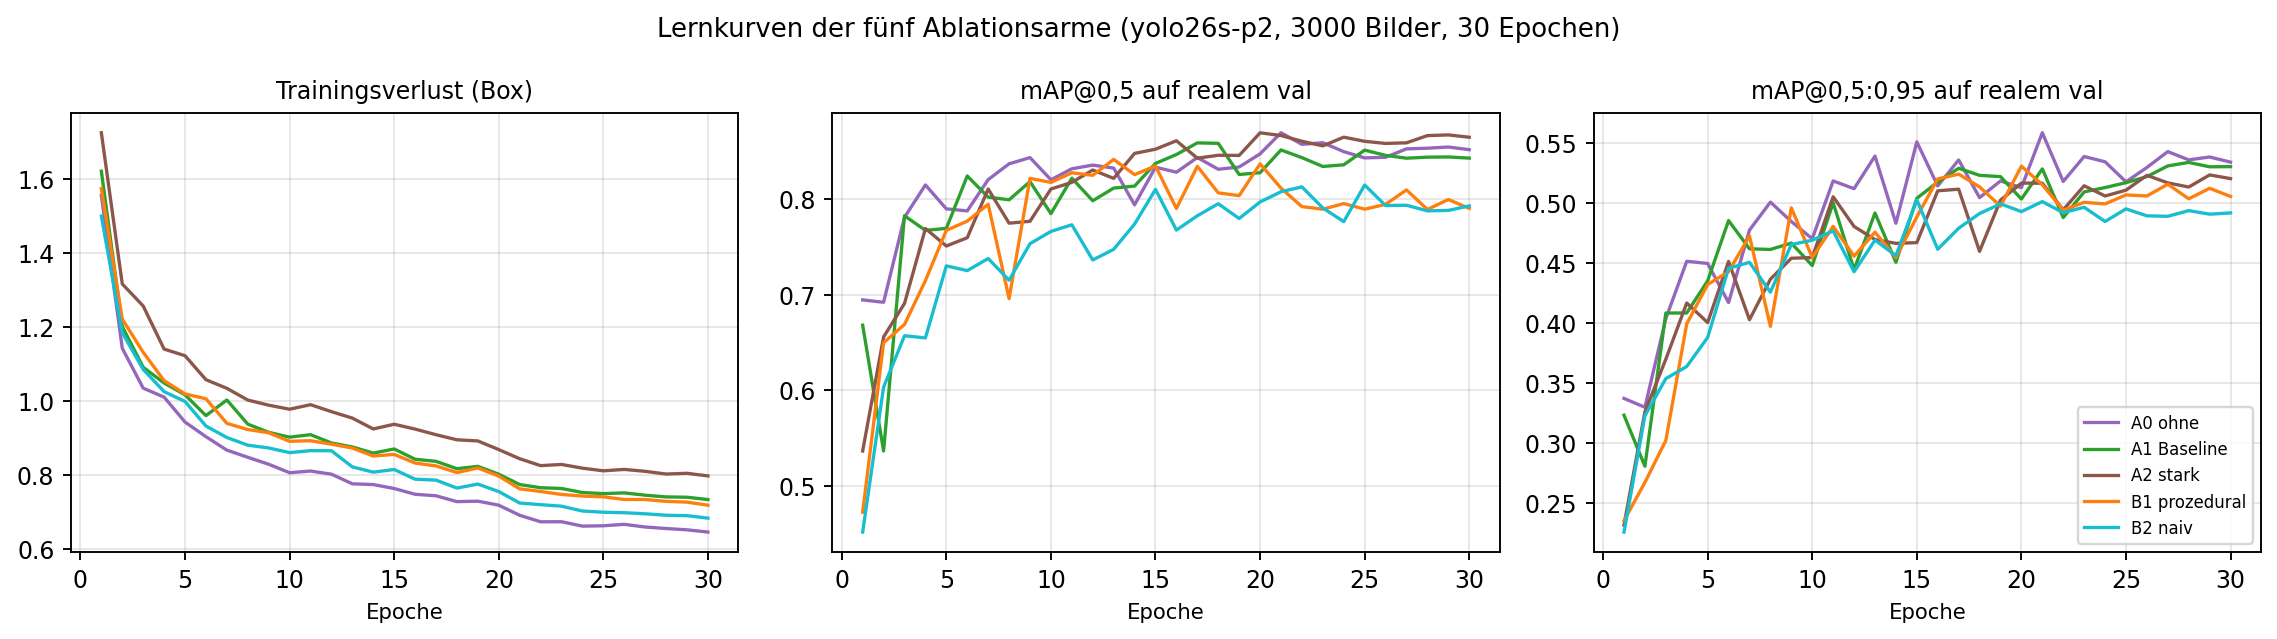
\includegraphics[width=\textwidth]{abbildungen/neu_training.png}\\[0.2em]
Referenzmodell: Early Stopping nach \zrefEpochen{} von 60 Epochen, bestes
Modell aus Epoche \zrefBestEpoche.
\end{column}
\begin{column}{0.49\textwidth}
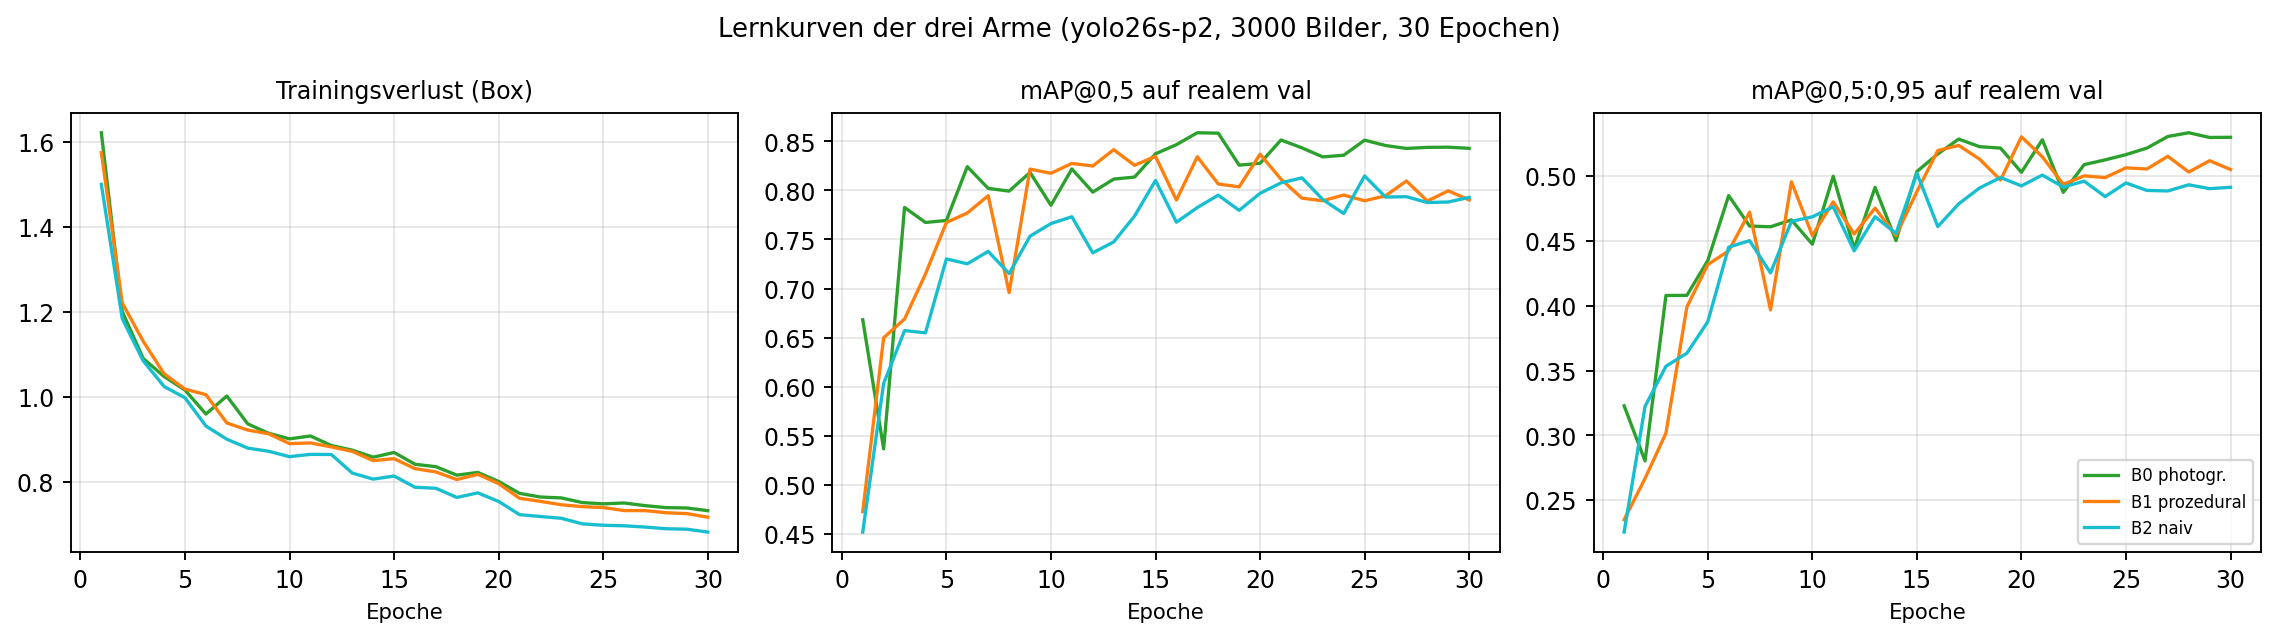
\includegraphics[width=\textwidth]{abbildungen/neu_training_b.png}\\[0.2em]
Die drei Ablationsarme, je 30 Epochen.
\end{column}
\end{columns}
\smallskip
{\color{akzent}Der Nebenbefund: B2 ist in Epoche \zBTwoEpoche{} austrainiert,
B1 in \zBOneEpoche, B0 erst in \zBZeroEpoche{} -- und B2 hat zugleich den
\emph{niedrigeren} Trainingsverlust. Beides sagt dasselbe: Der Trainingssatz
stellt eine leichtere Aufgabe, und die verbleibenden Epochen tragen nichts
mehr bei. Das ist die zeitliche Form des Befunds, dass starke Augmentierung
und kurzes Training nicht zusammenpassen -- der Erwartungswert in der
Risikogleichung wird praktisch durch \emph{eine} Ziehung je Bild und Epoche
genähert.}
\end{frame}

\begin{frame}{Z25 -- Qualitativergebnis}
\zusatzdicht
\begin{columns}[T,onlytextwidth]
\begin{column}{0.605\textwidth}
  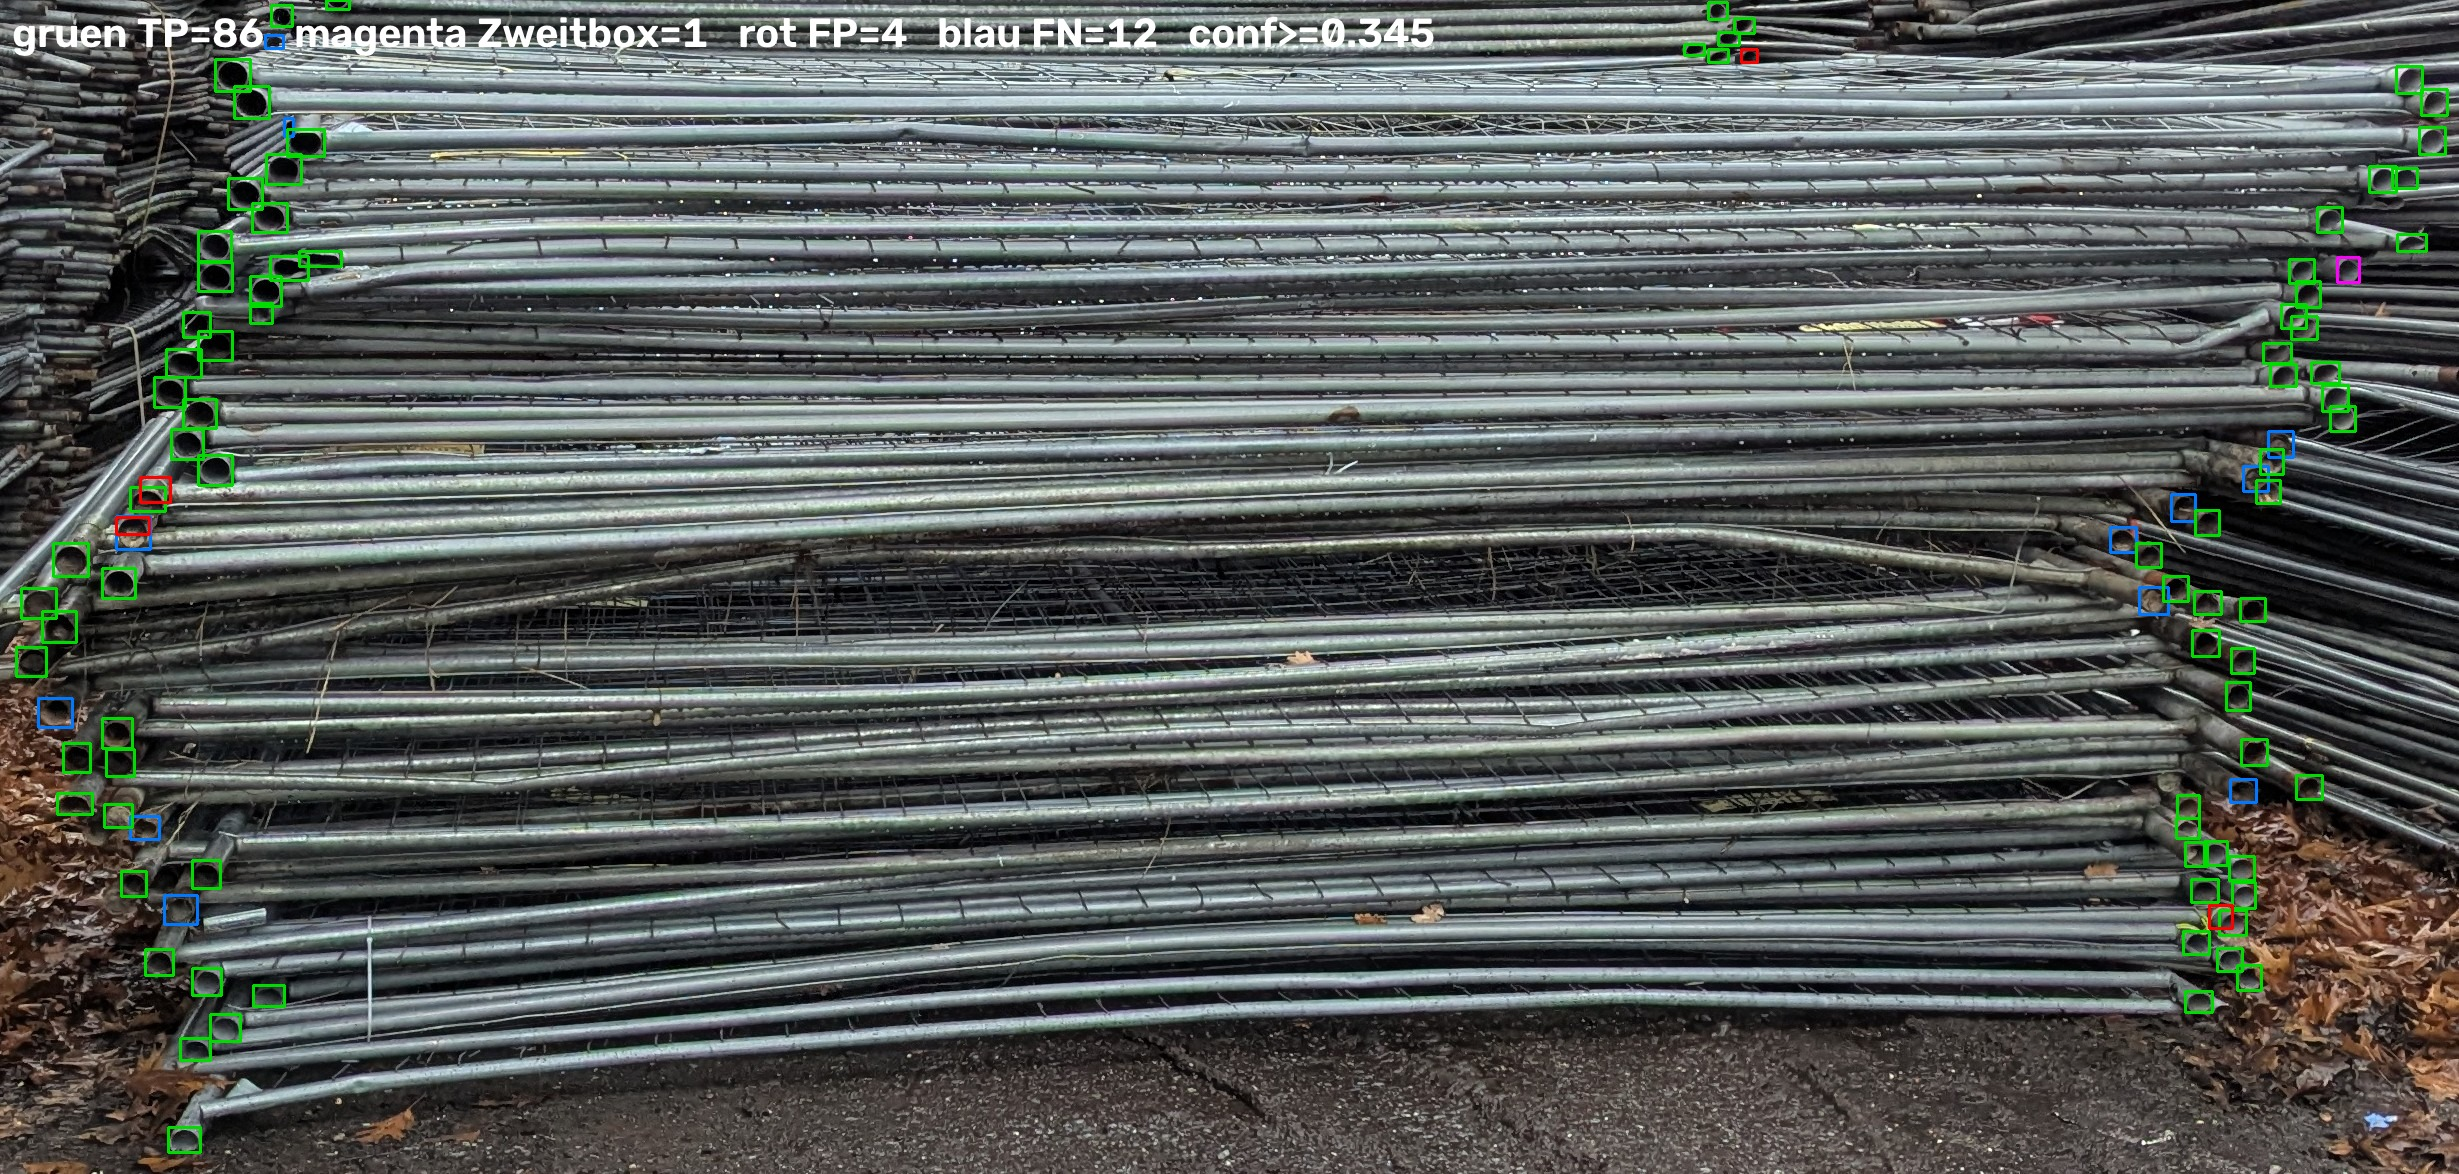
\includegraphics[width=\textwidth]{abbildungen/neu_qual_val.jpg}\\[0.15em]
  \code{val} -- $2459\times1174$, 98 Objekte, Median 26{,}8\px
\end{column}
\begin{column}{0.385\textwidth}
  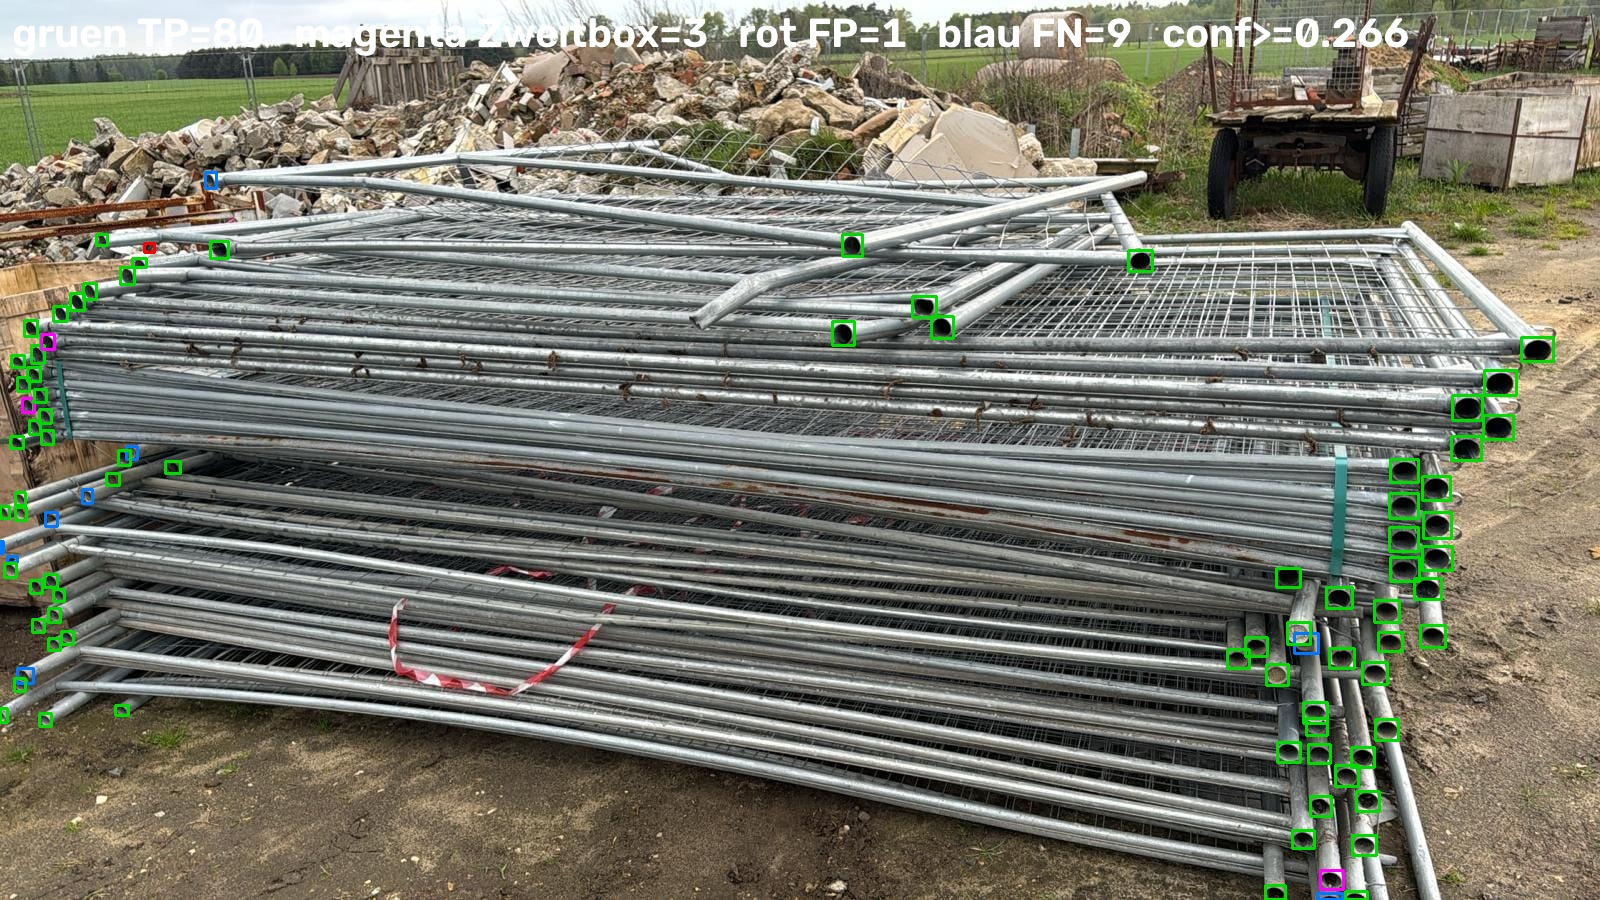
\includegraphics[width=\textwidth]{abbildungen/neu_qual_test.jpg}\\[0.15em]
  \code{test} -- $1600\times900$, 89 Objekte, Median 17{,}0\px{} -- der
  \emph{schwierigere} Split: kleinere Objekte, lockerere Packung, 6{,}7\,\%
  angeschnittene Boxen. Und der einzige, der Training und Modellauswahl nie
  berührt hat.
\end{column}
\end{columns}
\smallskip
Am $F_1$-optimalen Betriebspunkt. Auf \code{test}: \znPredTest{}
Detektionen, \zfpTest{} nicht auf einem annotierten Objekt, \zfnTest{}
übersehen.
\end{frame}

\end{document}
